% !TeX program = xelatex
\documentclass{beamer}
\usepackage{xeCJK}
\usepackage{bookmark}
% 图片路径
\graphicspath{{Figures/}}
% 设置主题
\usetheme{Berkeley}
\usecolortheme{beaver}
\setbeamercolor{title in sidebar}{fg=black}
\setbeamercolor{section in sidebar shaded}{fg=black}
\usefonttheme{serif}
% 报告基本信息
\logo{
\includegraphics[height=0.09\textwidth]{whulogo.eps}}
\title[Graph Embedding]{图表示学习}
\author[S. Zhou]{Zhou Shen}
\institute{School of Computer Science, Wuhan University}
\date{\today}

\begin{document}
% -----------------------------------------首页-----------------------------------------
\begin{frame}
    \titlepage
\end{frame}
% ----------------------------------------目录页----------------------------------------
\begin{frame}{Outline}
    \tableofcontents
\end{frame}
% ---------------------------------------Word2Vec---------------------------------------
\section{Word2Vec}
% 统计语言模型
\begin{frame}{Word2Vec}
    \framesubtitle{统计语言模型}
    对于一个给定的句子:
    $$S=\{w_1, w_2, w_3, w_4, \cdots, w_n\}$$
    其概率可以计算为:
    $$
        \begin{aligned}
            P(S)&=P\left(w_{1}, w_{2}, \ldots, w_{n}\right) \\
            &=P\left(w_{1}\right) P\left(w_{2} \mid w_{1}\right) \ldots P\left(w_{n} \mid w_{1}, w_{2}, \ldots, w_{n-1}\right) \\
            &=\prod_{i=1}^{n} p\left(w_{i} \mid w_{1} \ldots w_{i-1}\right)
        \end{aligned}
    $$
    缺点:1.数据稀疏严重 2.参数空间过大
\end{frame}

\begin{frame}{Word2Vec}
    \framesubtitle{N-Gram}
    马尔科夫假设:语言中的每一个词只与前面长度为$n-1$的上下文相关 \\
    例如:2-Gram模型假设下一个词的出现只依赖于前一个词
    $$P(S)=P(w_1)P(w_2 \mid w_1) \cdots P(w_n\mid w_{n-1})$$
    \begin{enumerate}[1)]
        \item 当n较大时,可以学习到更多语境信息,但是参数多,训练量大,更稀疏
        \item 当n较小时,提供的语境信息少,参数少,但是在训练语料库中出现的次数多,统计结果更加可靠
    \end{enumerate}
\end{frame}
% one-hot encoding
\begin{frame}{Word2Vec}
    \framesubtitle{One-Hot Encoding}
    \begin{columns}
        \begin{column}{0.5\textwidth}
            \centering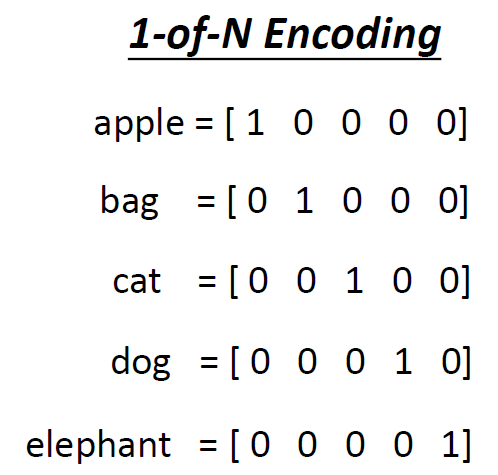
\includegraphics[height=5cm]{one_hot.png}
        \end{column}
        \begin{column}{0.5\textwidth}
            缺点:
            \begin{itemize}
                \item 单词的维度受到语料库的大小影响
                \item 相近的两个词的向量无法体现其关系
            \end{itemize}
        \end{column}
    \end{columns}
\end{frame}
% one-word context
\begin{frame}{Word2Vec}
    \framesubtitle{One-Word Context}
    \centering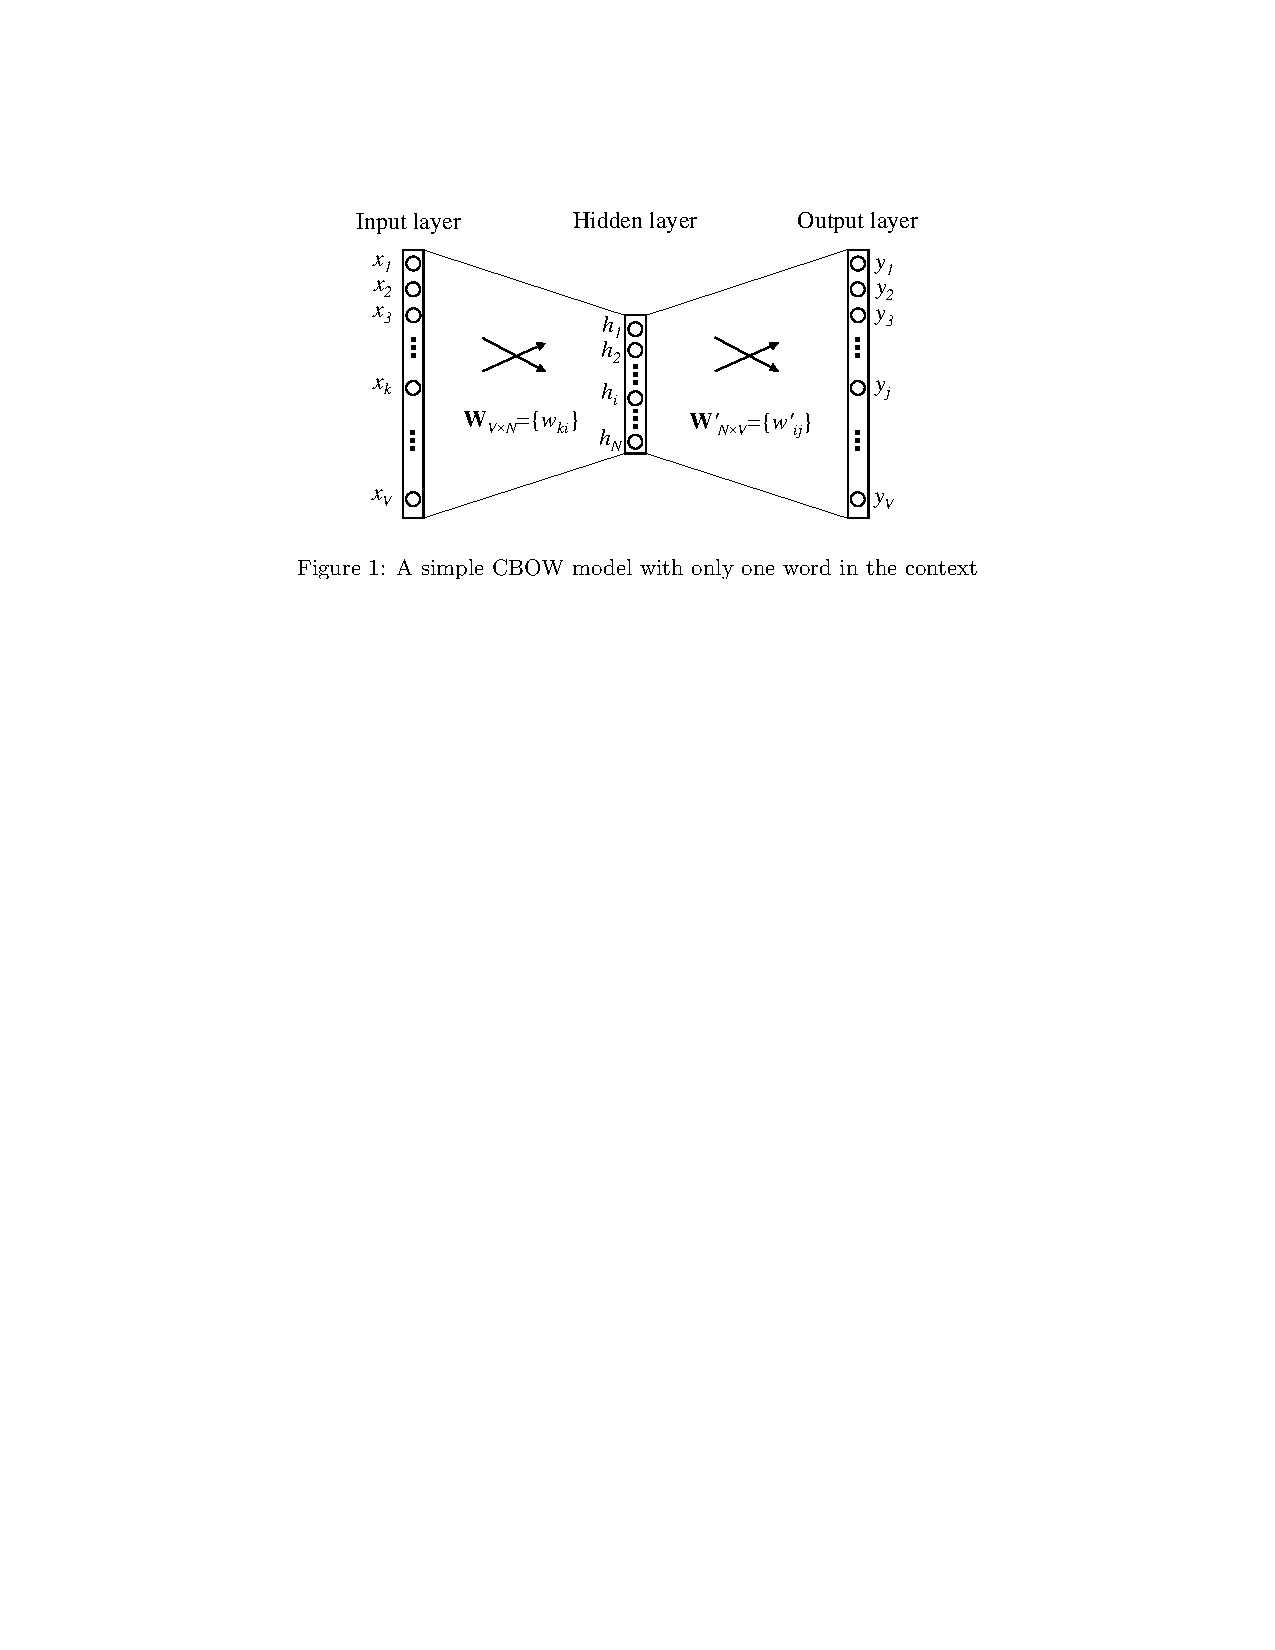
\includegraphics[height=4cm]{word2vec_1.pdf}
    $$
        \mathbf{h}=\mathbf{W}^{T} \mathbf{x}=\mathbf{W}_{(k, \cdot)}^{T}:=\mathbf{v}_{w_{I}}^{T}, u_j=\mathbf{v}_{w_j}^{\prime}h
    $$
    $$
        p\left(w_{j} \mid w_{I}\right)=y_{j}=\frac{\exp \left(u_{j}\right)}{\sum_{j^{\prime}=1}^{V} \exp \left(u_{j^{\prime}}\right)}
        $$
\end{frame}
% Objective Function
\begin{frame}{Word2Vec}
    \framesubtitle{Objective Function}
    \begin{equation}
        \begin{aligned}
            \max p\left(w_{O} \mid w_{I}\right) &=\max y_{j^{*}} \\
            &=\max \log y_{j^{*}} \\
            &=u_{j^{*}}-\log \sum_{j^{\prime}=1}^{V} \exp \left(u_{j^{\prime}}\right):=-E
            \end{aligned}
    \end{equation}
    \begin{alertblock}{常用变形}
        $\min E=-u_{j^{*}}+\log \sum_{j^{\prime}=1}^{V} \exp \left(u_{j^{\prime}}\right)$
    \end{alertblock}
\end{frame}
% CBOW
\begin{frame}{Word2Vec}
    \framesubtitle{CBOW}
    \begin{columns}
        % 第一列
        \begin{column}{0.4\textwidth}
            \centering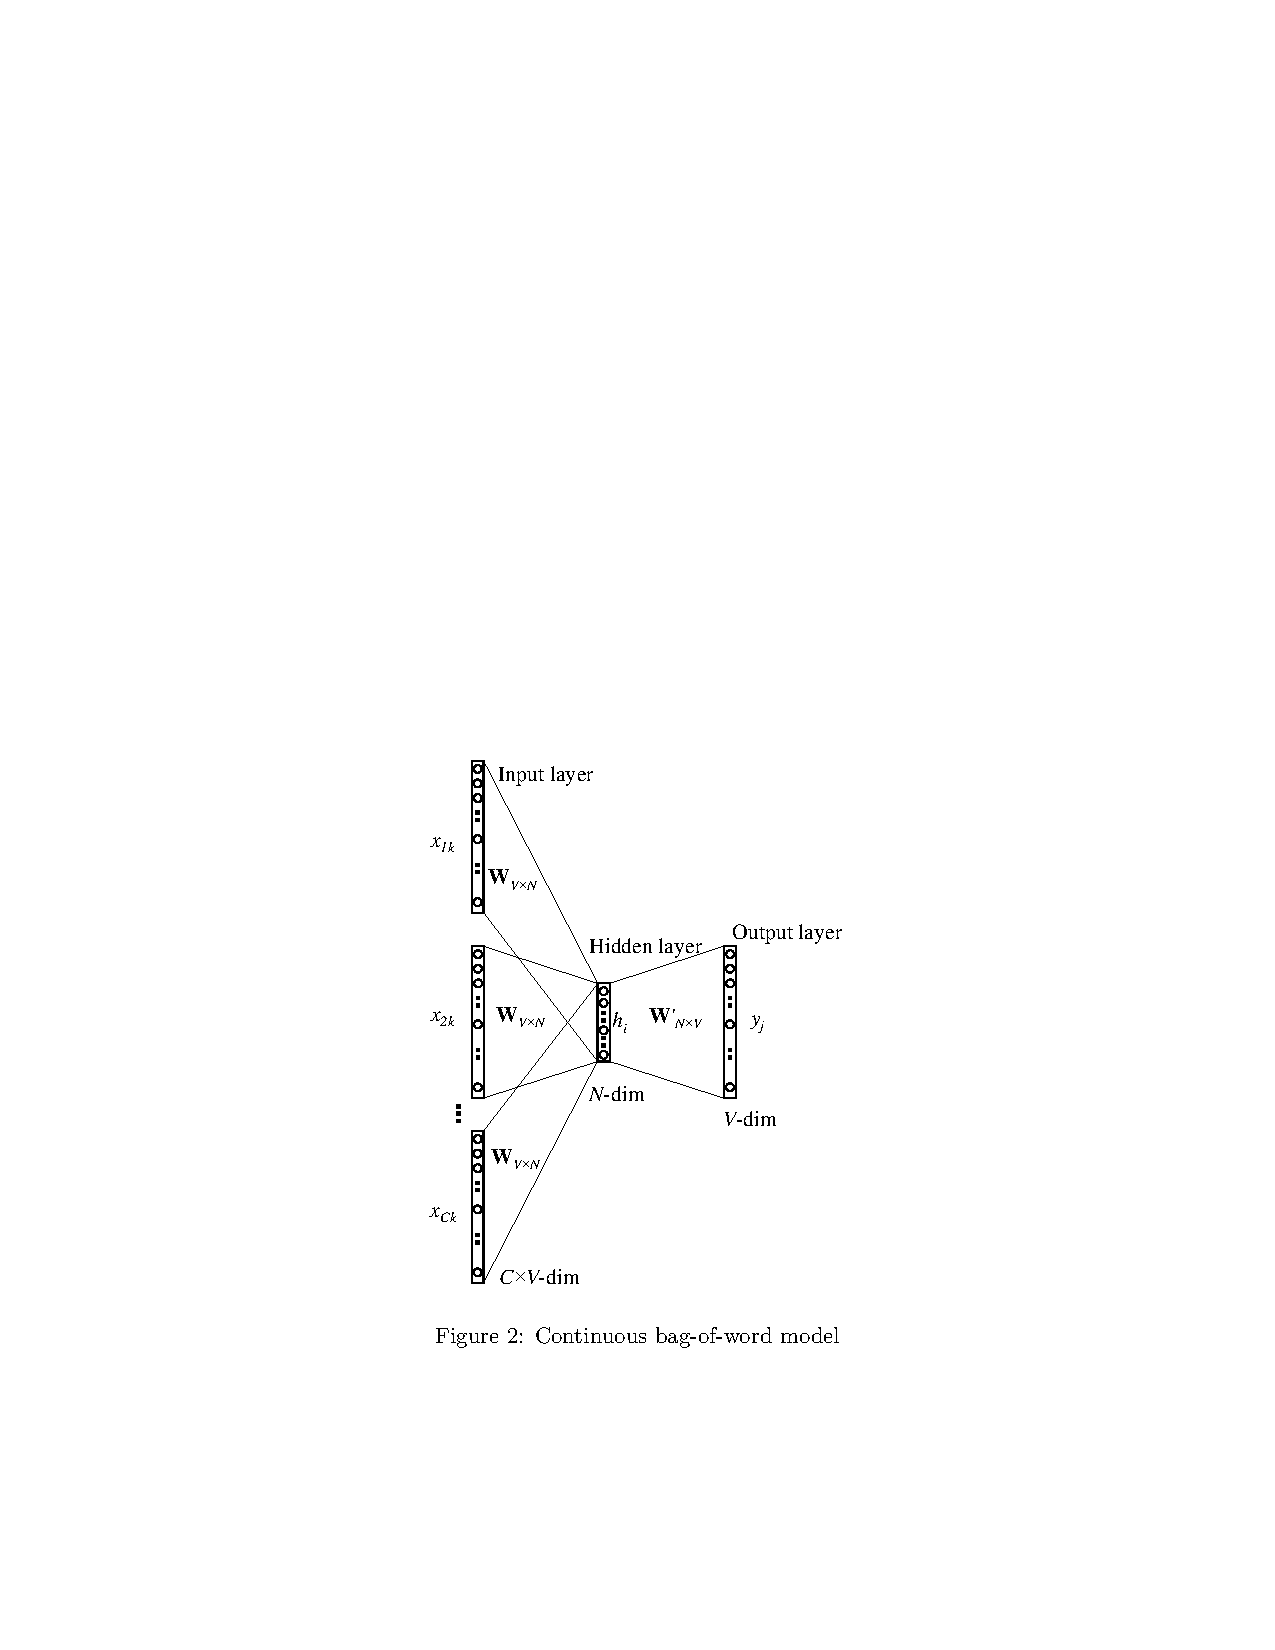
\includegraphics[height=6cm]{word2vec_2.pdf}
        \end{column}
        % 第二列
        \begin{column}{0.6\textwidth}
            $$\mathbf{h} = \frac{1}{C}(\mathbf{v}_{w_1} + \mathbf{v}_{w_2} + \cdots + \mathbf{v}_{w_C})^T$$
            $$
            \begin{aligned}
                E &=-\log p\left(w_{O} \mid w_{I, 1}, \cdots, w_{I, C}\right) \\
                &=-u_{j^{*}}+\log \sum_{j^{\prime}=1}^{V} \exp \left(u_{j^{\prime}}\right) \\
            \end{aligned}
            $$
        \end{column}
    \end{columns}
\end{frame}
% Skip-Gram
\begin{frame}{Word2Vec}
    \framesubtitle{Skip-Gram}
    \begin{columns}
        % 第一列
        \begin{column}{0.4\textwidth}
            \centering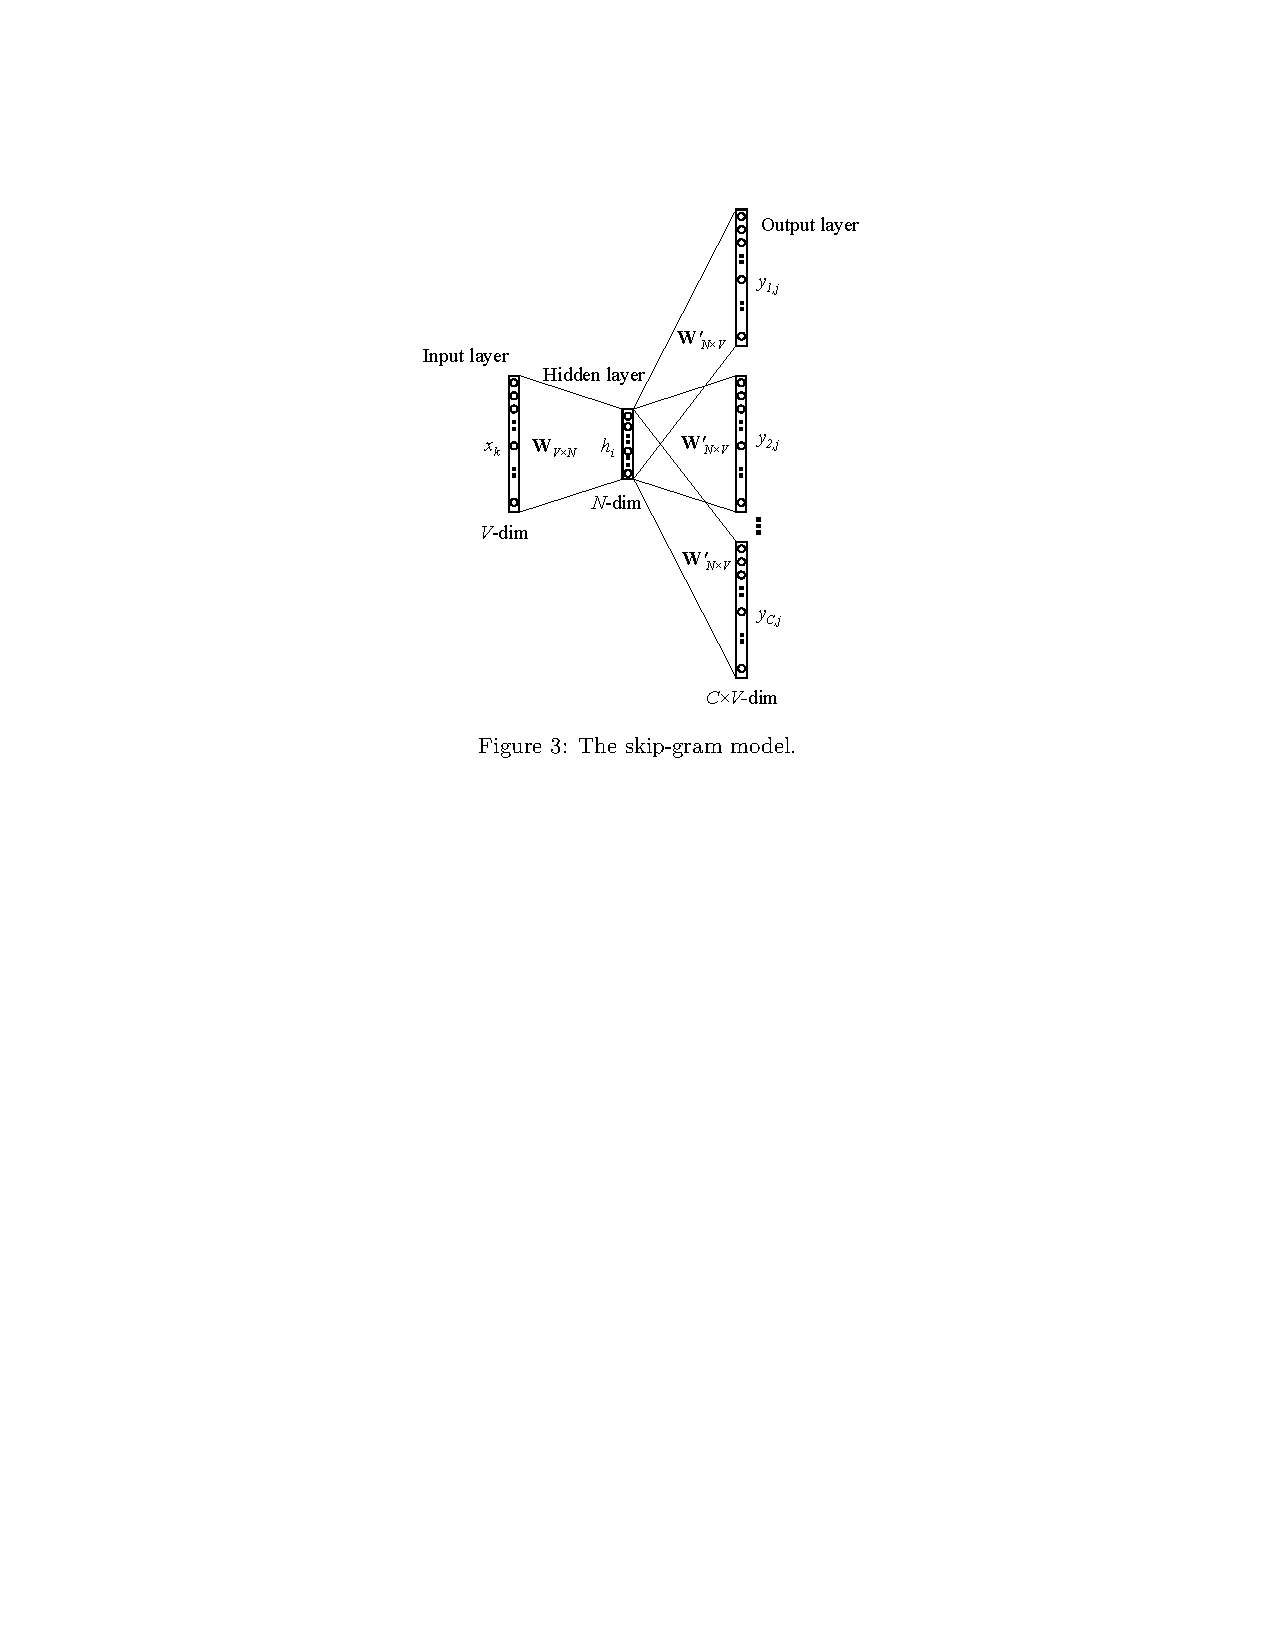
\includegraphics[height=6cm]{word2vec_3.pdf}
        \end{column}
        % 第二列
        \begin{column}{0.6\textwidth}
            $$
            \begin{aligned}
            E &=-\log p\left(w_{O, 1}, w_{O, 2}, \cdots, w_{O, C} \mid w_{I}\right) \\
            &=-\log \prod_{c=1}^{C} \frac{\exp \left(u_{c, j_{c}^{*}}\right)}{\sum_{j^{\prime}=1}^{V} \exp \left(u_{j^{\prime}}\right)} \\
            &=-\sum_{c=1}^{C} u_{j_{c}^{*}}+C \cdot \log \sum_{j^{\prime}=1}^{V} \exp \left(u_{j^{\prime}}\right)
            \end{aligned}
            $$
        \end{column}
    \end{columns}
\end{frame}
% Hierarchical Softmax
\begin{frame}{Word2Vec}
    \framesubtitle{Hierarchical Softmax}
    哈夫曼树的构建是基于语料库中单词出现的频率
    \centering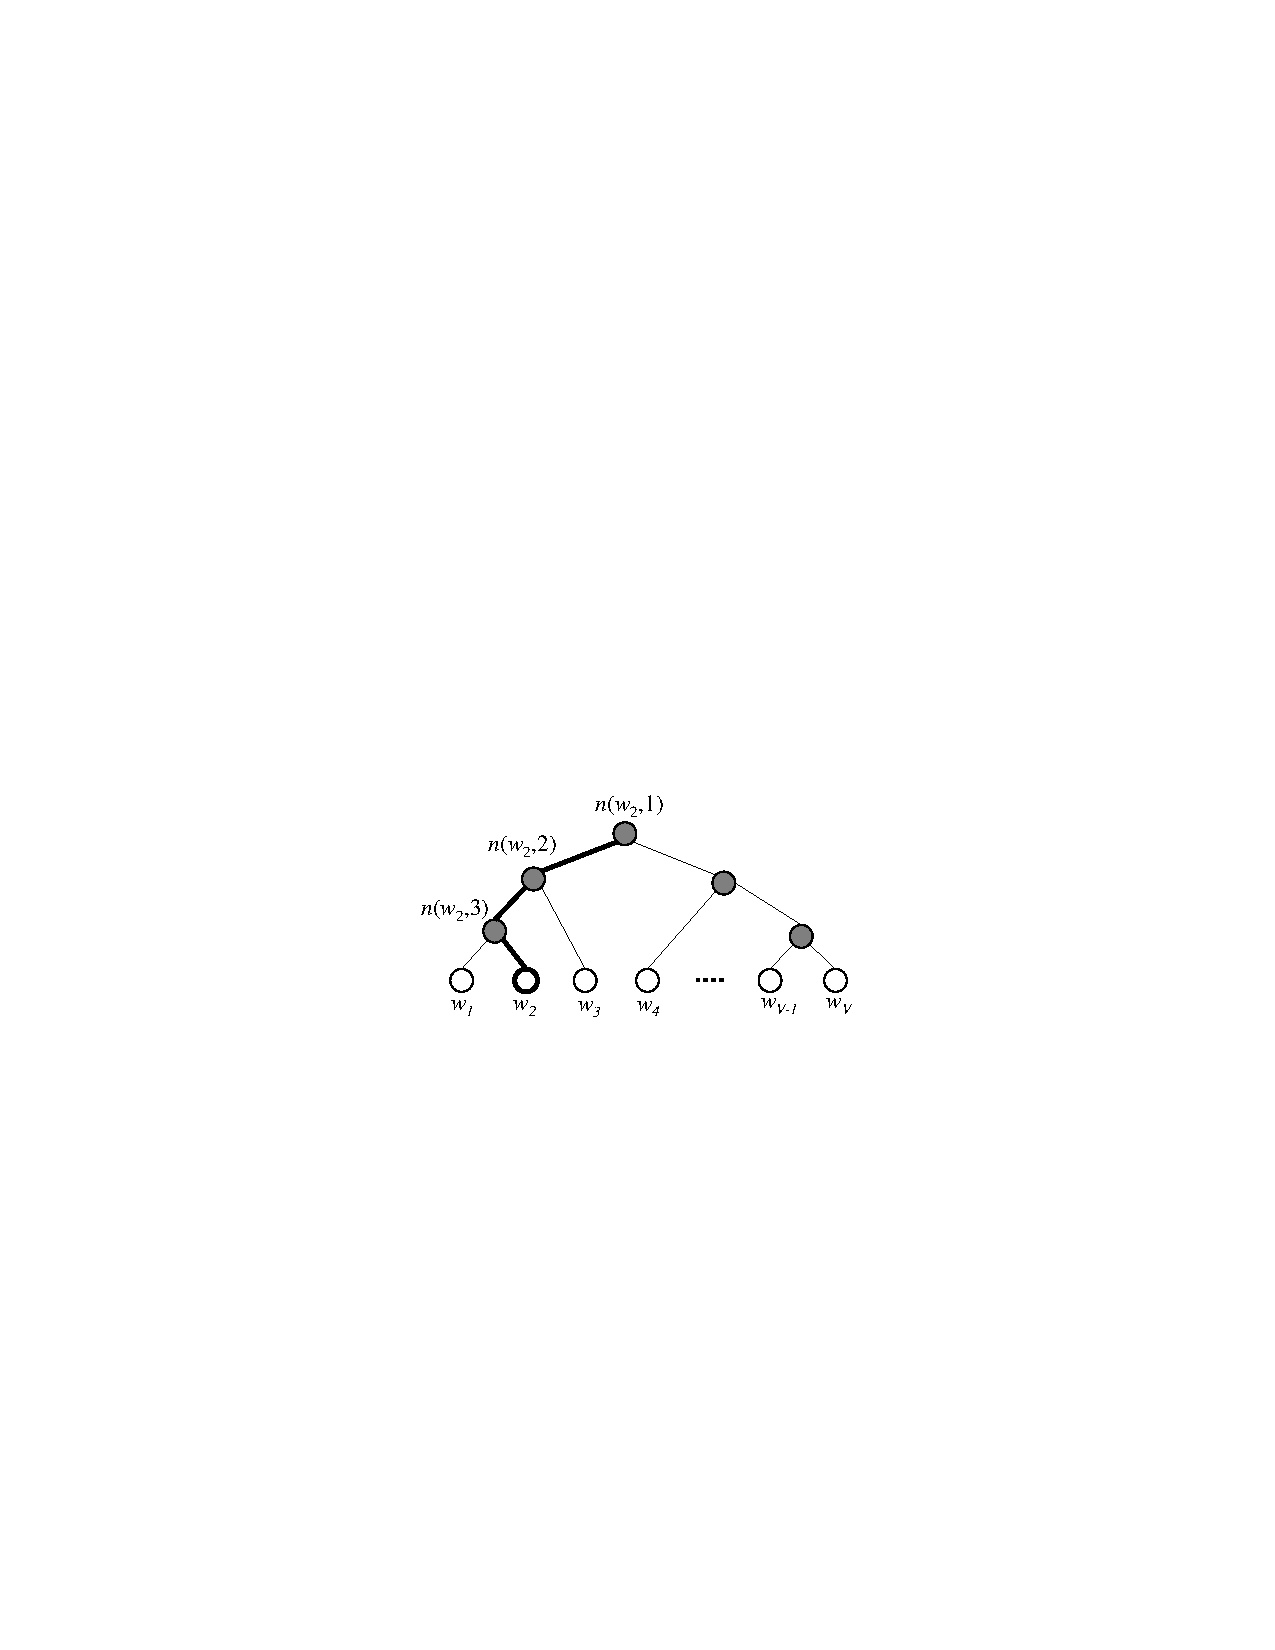
\includegraphics[height=4cm]{word2vec_4.pdf}
    $$
        p\left(w=w_{O}\right)=\prod_{j=1}^{L(w)-1} \sigma\left([ n(w, j+1)=\operatorname{ch}(n(w, j)) ] \cdot \mathbf{v}_{n(w, j)}^{\prime}{ }^{T} \mathbf{h}\right)
    $$
\end{frame}
% Negative Sample
\begin{frame}{Word2Vec}
    \framesubtitle{Negative Sample}
    1. 词频计算
    $$
        weight(w_i) = \frac{count(w_i)^{0.75}}{\sum_{j}^{V} count(w_j)^{0.75}}
    $$
    2. 目标函数
    $$
        E=-\log \sigma\left(\mathbf{v}_{w_{O}}^{\prime}{ }^{T} \mathbf{h}\right)-\sum_{w_{j} \in \mathcal{W}_{\mathrm{neg}}} \log \sigma\left(-\mathbf{v}_{w_{j}}^{\prime}{ }^{T} \mathbf{h}\right)
    $$
\end{frame}
% 总结
\begin{frame}{Word2Vec}
    \framesubtitle{总结}
    \begin{enumerate}
        \item Word2Vec主要包含两个模型CBOW(根据上下文预测中心词的概率)与Skip-Gram(根据中心词来预测上下文)
        \item Word2Vec可以被看作是一个多分类模型,但是我们更加关注这个模型的附加产物(每一个单词的映射向量)
        \item Hierarchical Softmax与Negative Sample其实本质上都是在优化softmax,我们知道softmax的时间复杂度是$O(N)$,
              因此,我们可以将其转化为$log(N)$次的二分类计算,这便是Hierarchical Softmax。负采样则是对(1)式的后半
              部分进行优化,不需要全部的非目标词都作为负样本,等于把$O(N)$复杂度降为$O(m)$,m为负样本的个数。
    \end{enumerate}
\end{frame}
% ---------------------------------------DeepWalk---------------------------------------
\section{DeepWalk}
% 问题定义
\begin{frame}{DeepWalk}
    \centering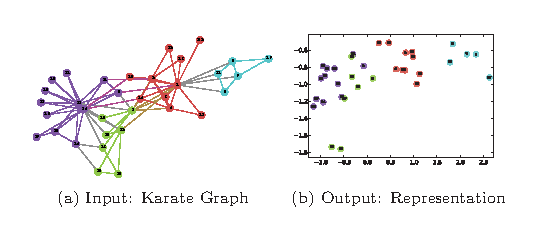
\includegraphics[height=3.8cm]{DeepWalk_1.eps}
    \begin{definition}{Problem Definition}
        Let $G = \left( V ,E \right)$, where $V$ are the members of the network, and $E$ be its edgs.
        Our goal is to learn $X_E\in \mathcal{R} ^{|V|\times d}$, where $d$ is number of 
        latent dimensions.
    \end{definition}
\end{frame}
% 为什么可以套用Word2Vec的思想
\begin{frame}{DeepWalk}
    \centering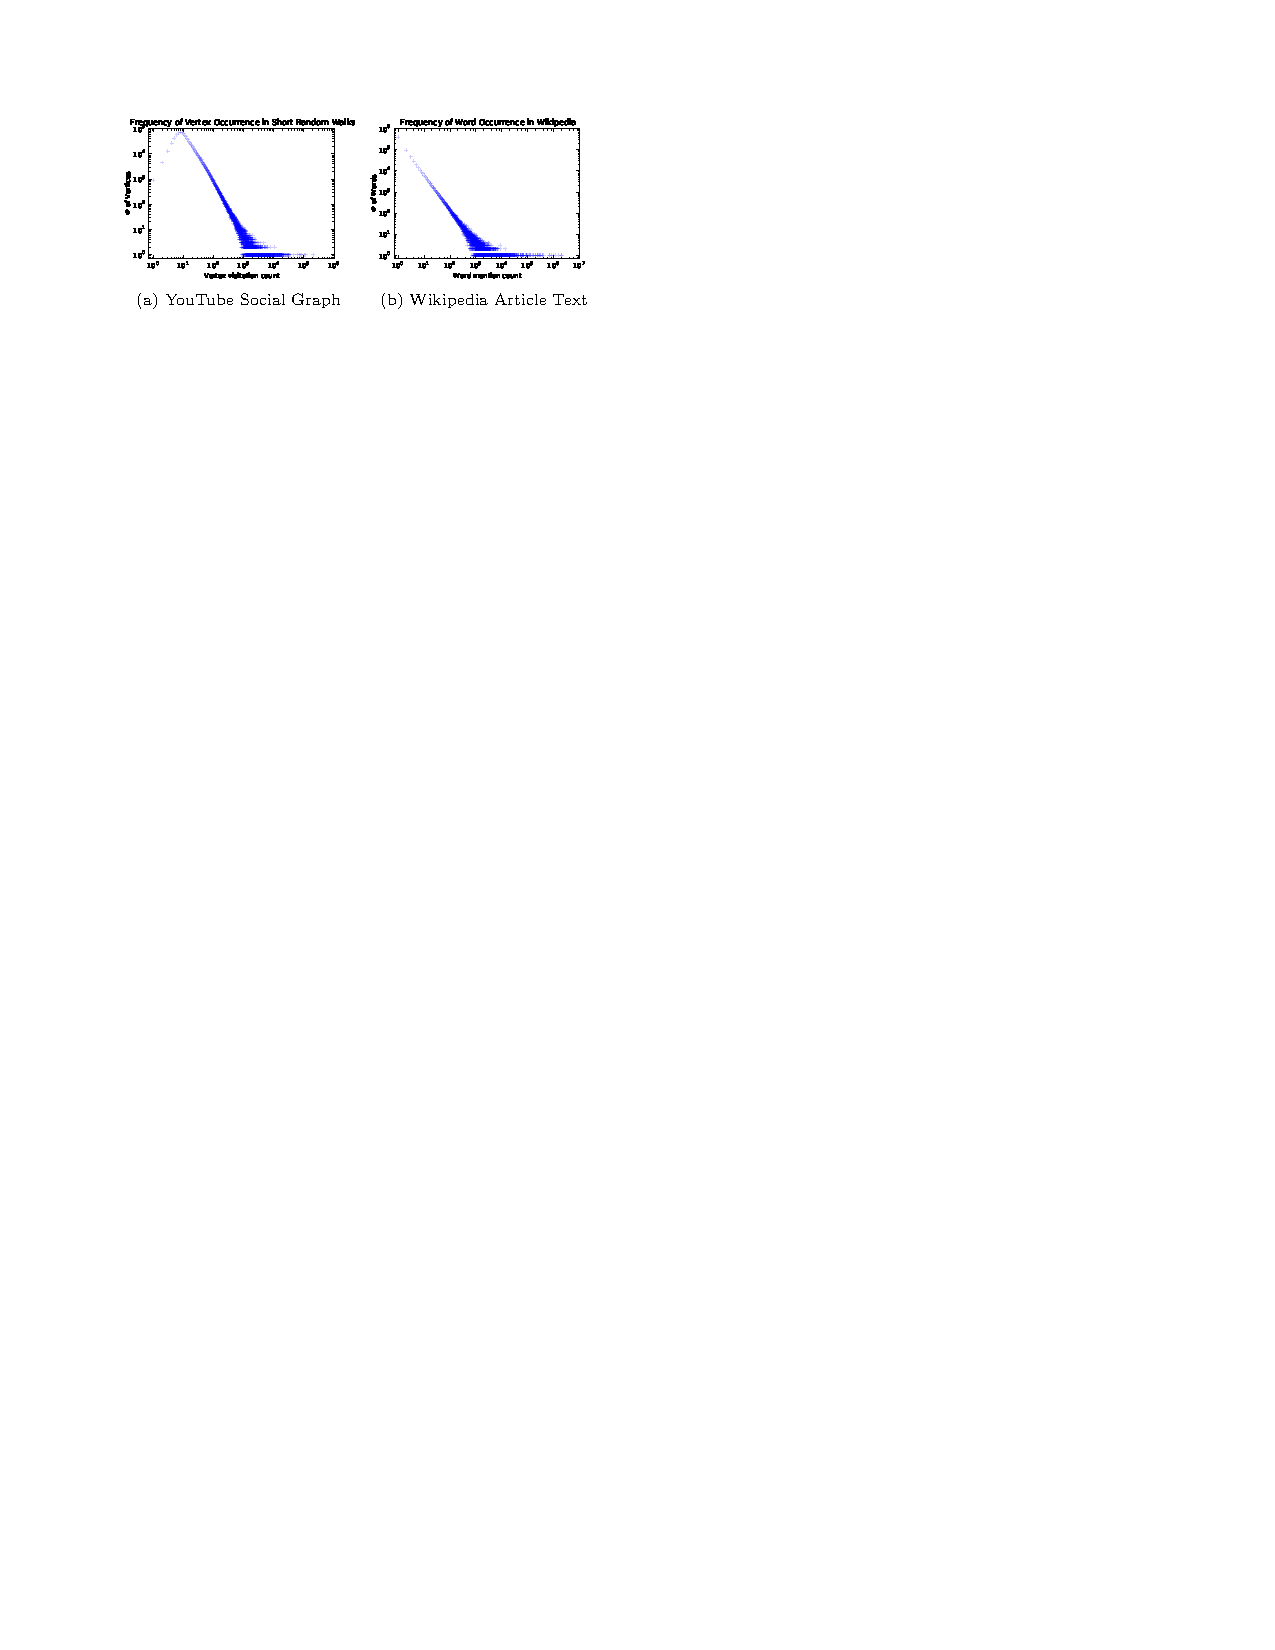
\includegraphics[height=4cm]{DeepWalk_2.pdf}
    \begin{alertblock}{Connection}
        The power-law distribution of vertices appearing in the short random walks follows 
        a power-law, much like the distribution of words in natural language.
    \end{alertblock}
\end{frame}
% 公式推导
\begin{frame}{DeepWalk}
    \begin{enumerate}
        \item give a sequence of random walk from vertice $i$
            \begin{equation}
                \mathcal{W}_{i}^{n}  = \{v_1, v_2, v_3, \cdots , v_n\}
            \end{equation}
        \item maximize the likehood
            \begin{equation}
                \operatorname{Pr}\left(v_i \mid \left(\Phi(v_1), \Phi(v_2), \cdots, \Phi(v_{i-1}))\right)\right)
            \end{equation}
            \begin{block}{Mapping Function $\Phi$}
                $\Phi: v \in V \longmapsto \mathcal{R}^{|V|\times d}$
                where $d$ is the number of dimensions                
            \end{block}
    \end{enumerate}
\end{frame}
% 为什么使用Skip-Gram
\begin{frame}{DeepWalk}
    \framesubtitle{Disadvantages and Optimizations}
    \begin{itemize}
        \item As the walk length grows, computing this objective function becomes unfeasible.
        \item Restricts the order in which vertices appear
    \end{itemize}
    \centering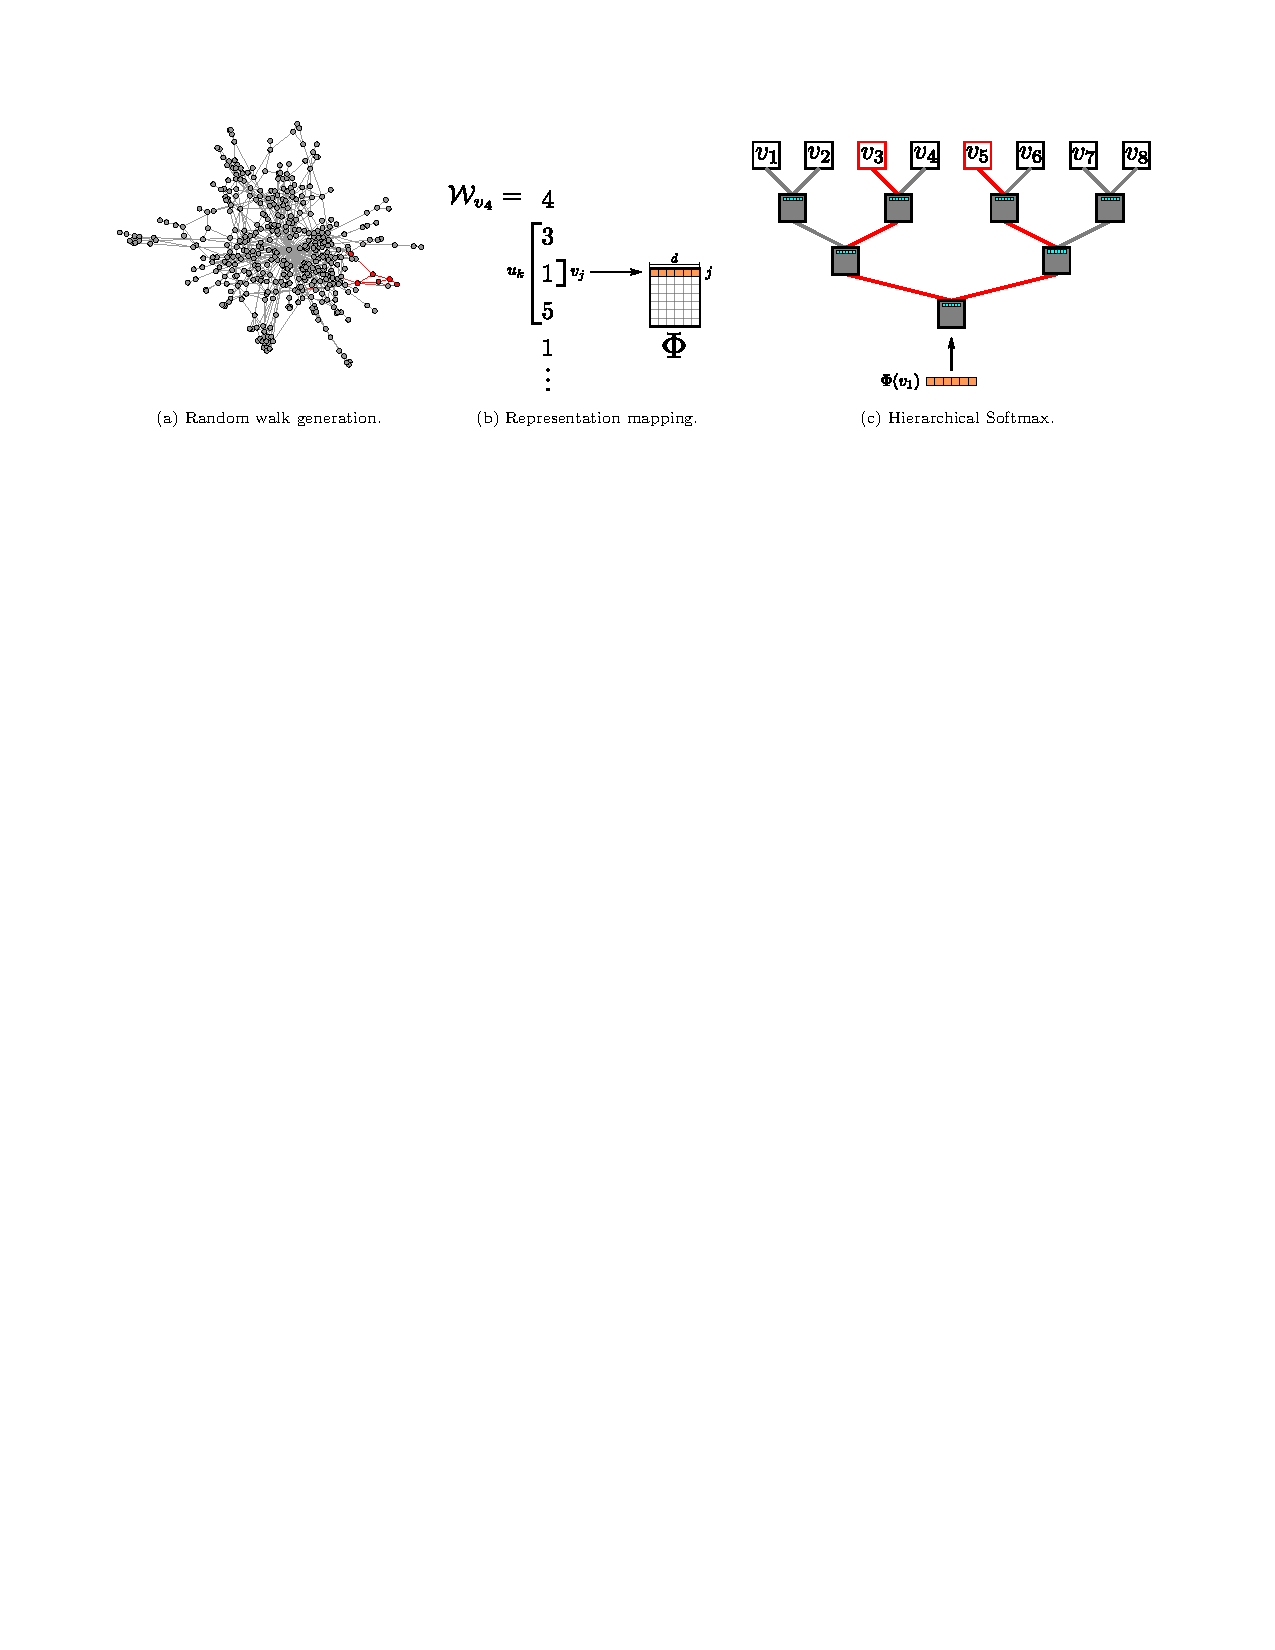
\includegraphics[height=3.1cm]{DeepWalk_3.pdf}
\end{frame}
% 优化目标与算法
\begin{frame}{DeepWalk}
    \framesubtitle{Algorithm}
    \centering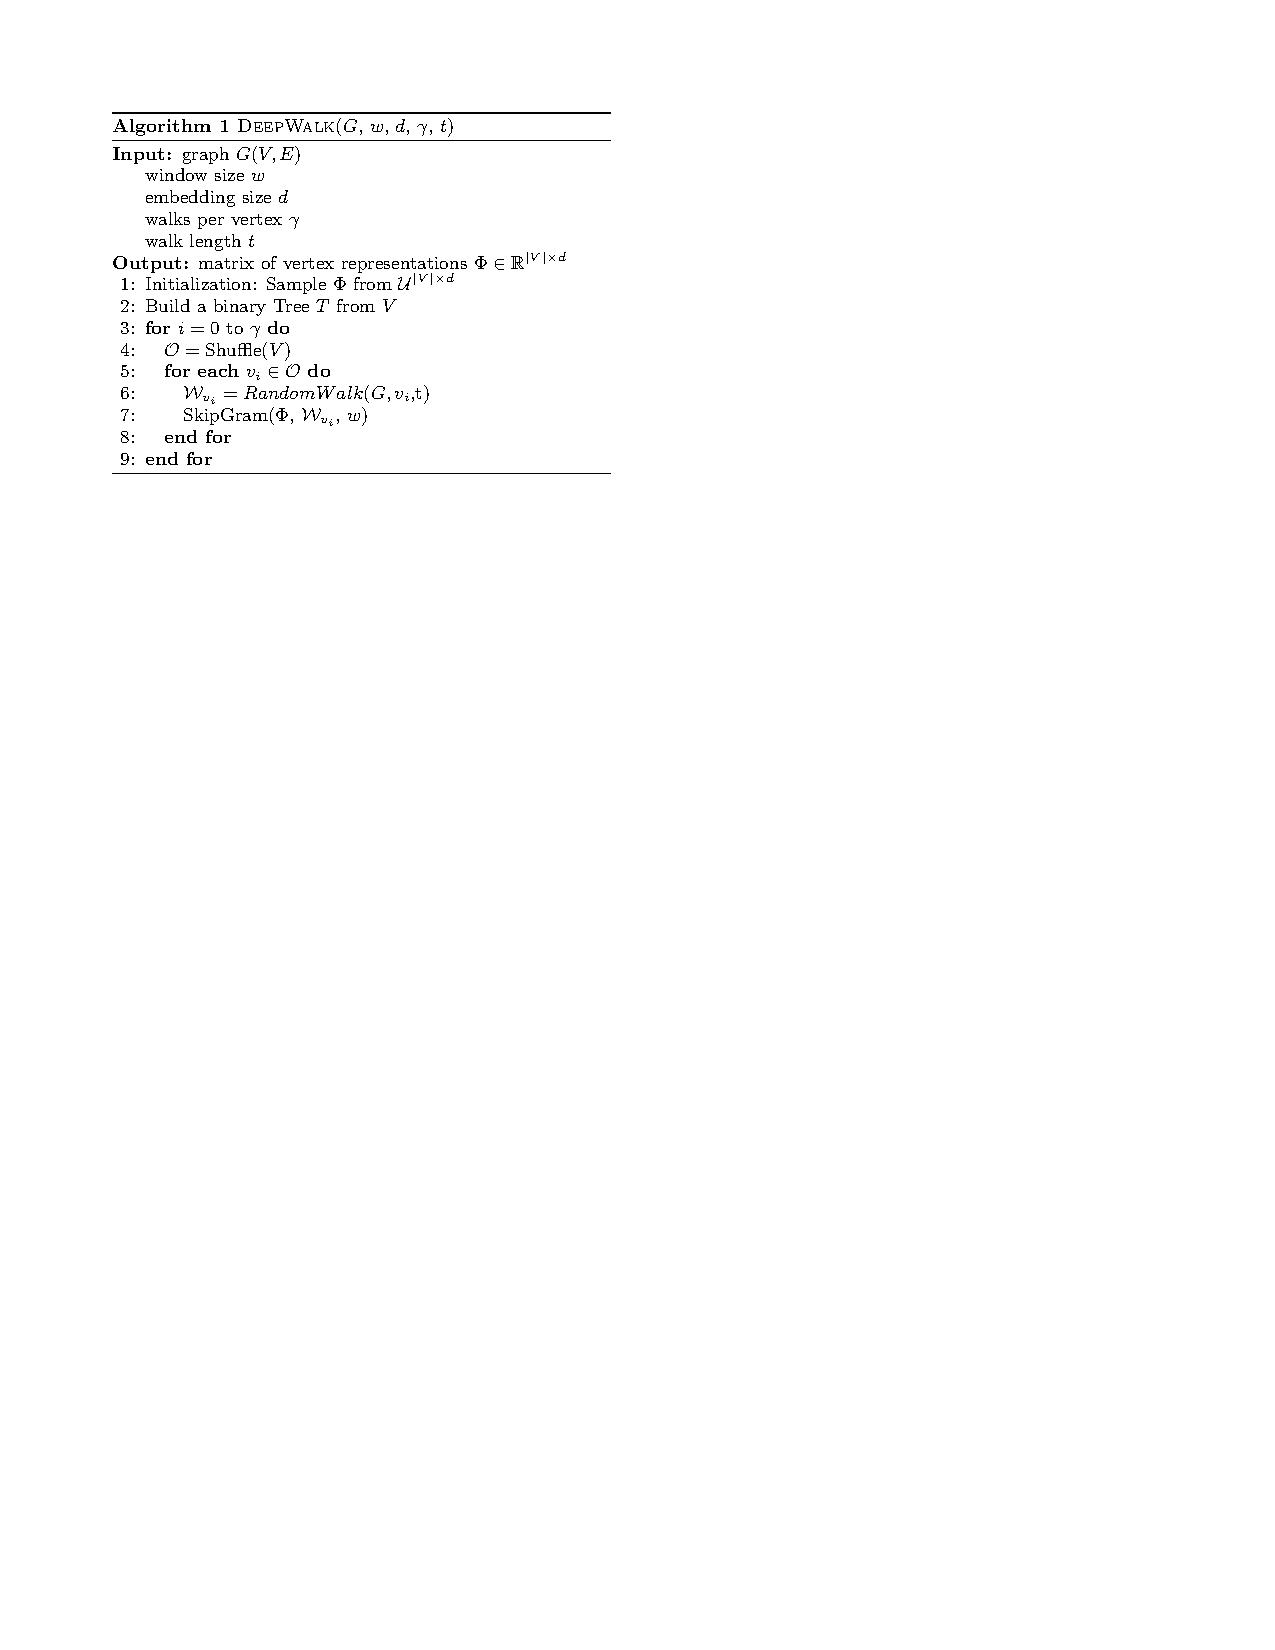
\includegraphics[height=5cm, width=7cm]{DeepWalk_4.pdf}
    \begin{corollary}
        $\underset{\Phi}{\operatorname{minimize}}-\log \operatorname{Pr}\left(\left\{v_{i-w}, \cdots, v_{i-1}, v_{i+1}, \cdots, v_{i+w}\right\} \mid \Phi\left(v_{i}\right)\right)$
    \end{corollary}
\end{frame}
% 总结
\begin{frame}{DeepWalk}
    \framesubtitle{总结}
    \begin{enumerate}
        \item DeepWalk将图中的每一个点对应成一个单词,将图中随机游走生成的序列看作是句子,基于此使用Work2Vec的思想来学习
              每一个节点的向量,并用作下游任务
        \item 正是由于其游走的随机性,DeepWalk没有确定的相似度优化目标函数,没有办法针对性的捕捉特定的相似性
        (homophily and structural equivalence)
    \end{enumerate}
\end{frame}
% ---------------------------------------Node2Vec---------------------------------------
\section{Node2Vec}
% 为什么使用BFS与DFS
\begin{frame}{Node2Vec}
    \framesubtitle{Classic Search Strategies}
    \centering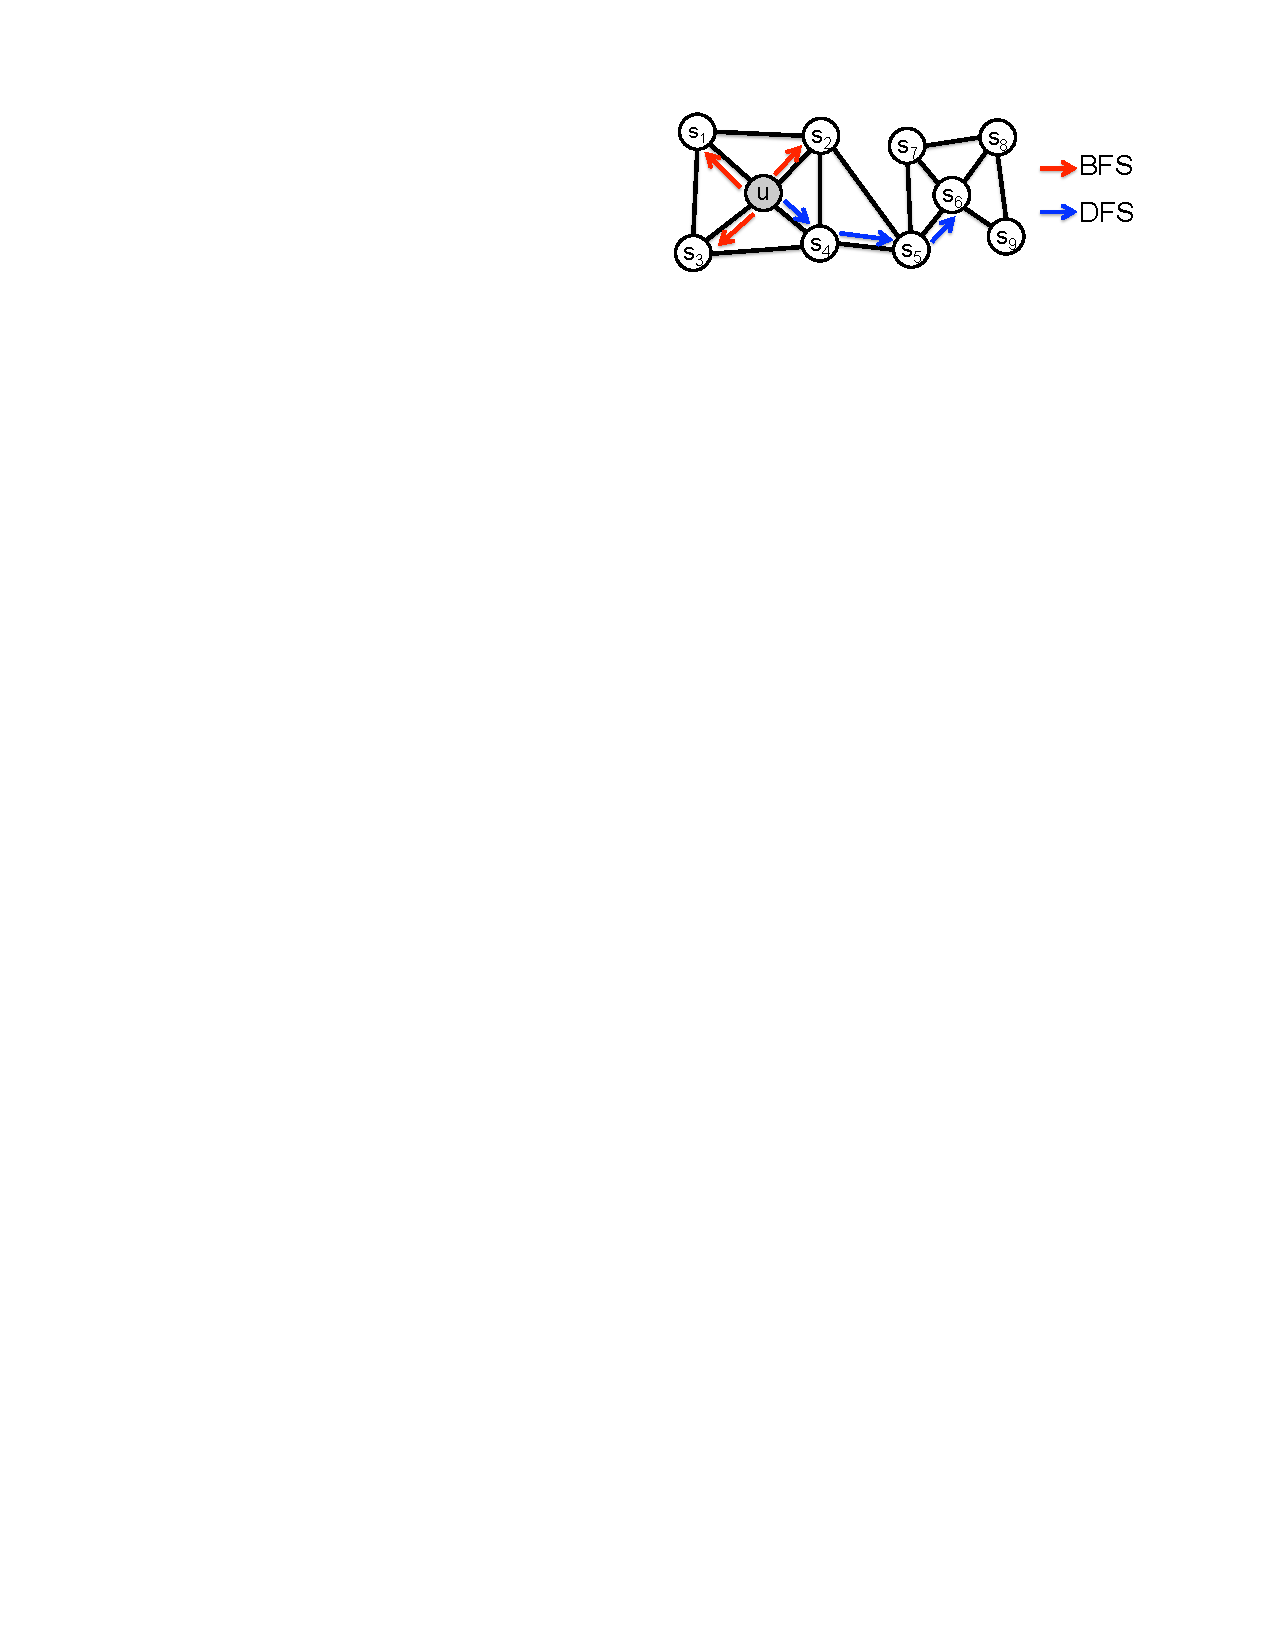
\includegraphics[height=3.8cm]{node2vec_1.pdf}
    1. The neighborhoods sampled by BFS lead to embeddings that correspond closely to structural equivalence.\\
    2. DFS can freely explore network neighborhoods which is important in discovering homophilous communities.
\end{frame}
% 如何控制BFS与DFS
\begin{frame}{Node2Vec}
    \framesubtitle{Search Bias $\alpha$ }
    \begin{columns}
        \begin{column}{0.5\textwidth}
            \centering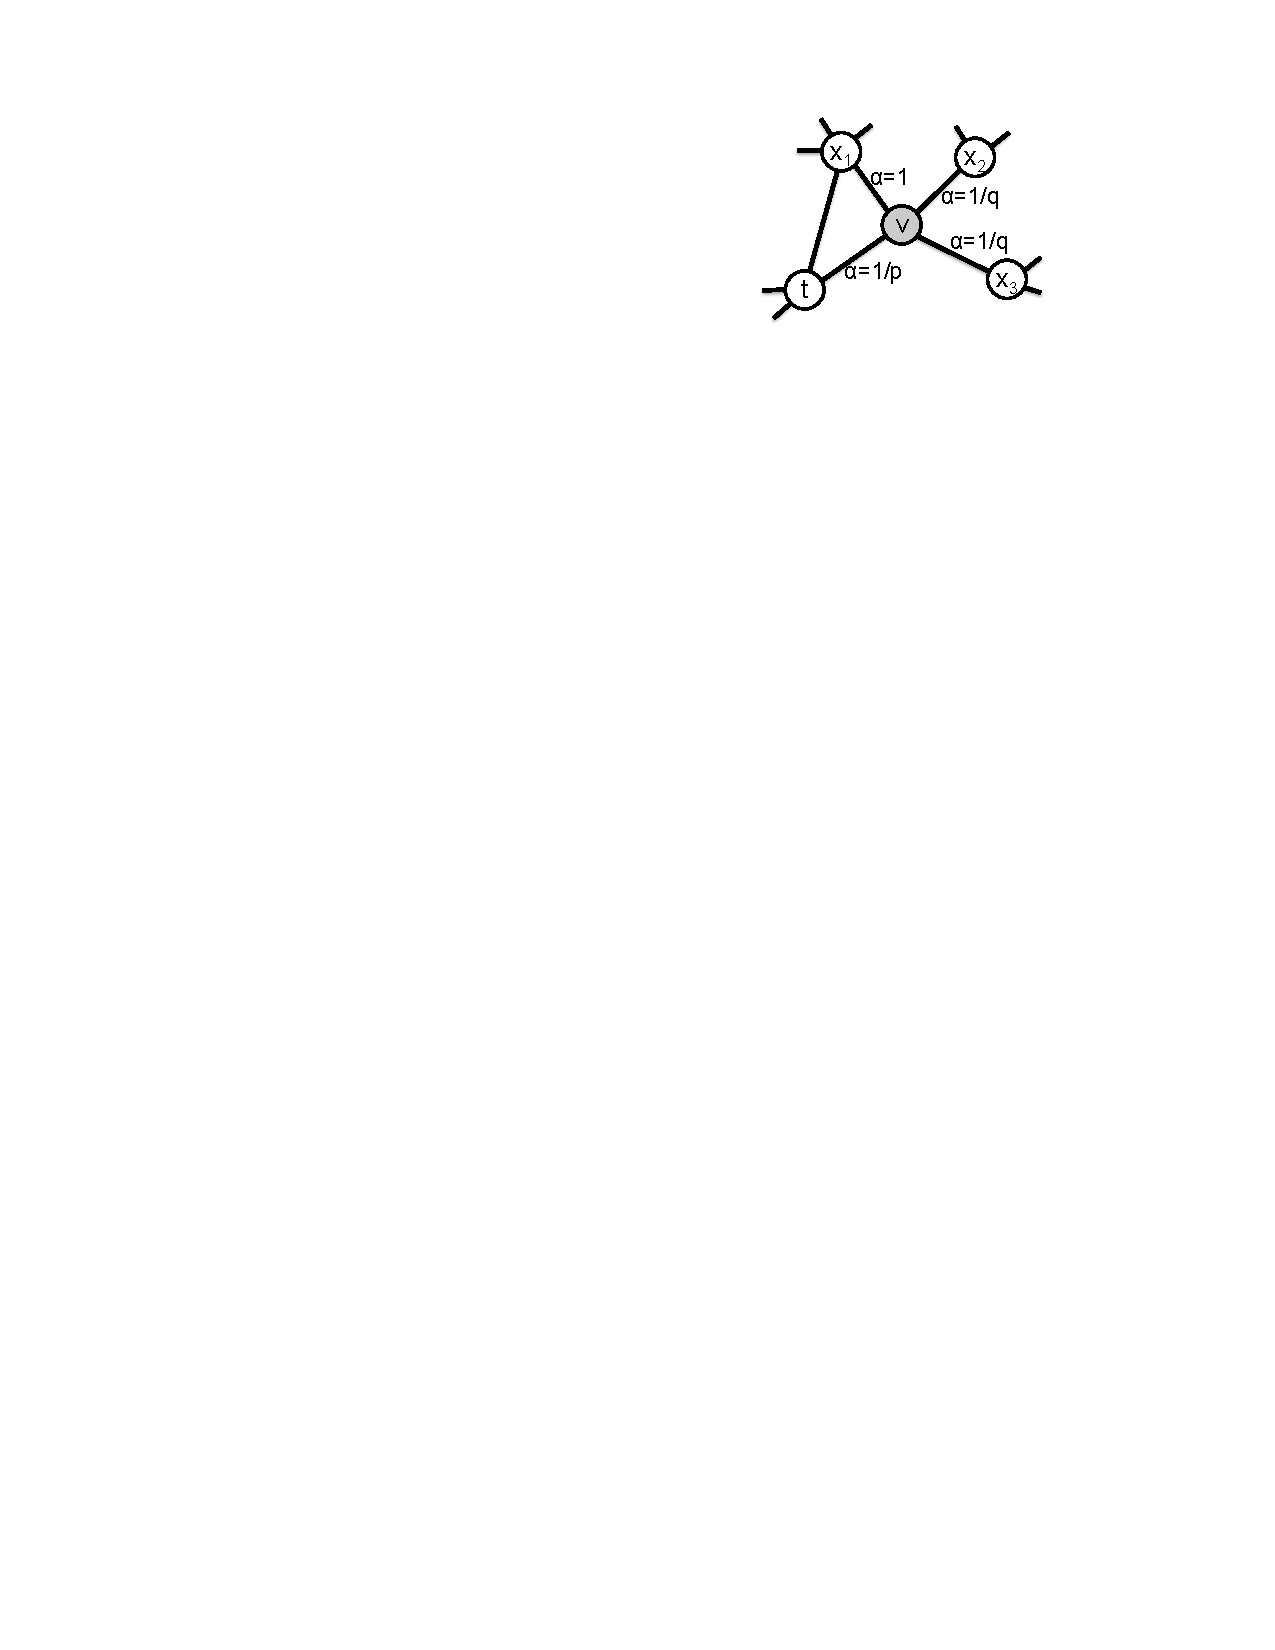
\includegraphics[height=3.6cm]{node2vec_2.pdf}
        \end{column}
        \begin{column}{0.5\textwidth}
            $$
            \alpha_{p q}(t, x)= \begin{cases}\frac{1}{p} & \text { if } d_{t x}=0 \\ 1 & \text { if } d_{t x}=1 \\ \frac{1}{q} & \text { if } d_{t x}=2\end{cases}
            $$
        \end{column}
    \end{columns}
    这里表示的是当上一个经过的点是$t$,且当前位于$v$,则下一个点转移的影响因子$\alpha $的计算公式,转移权重公式为$\pi_{v x}=\alpha_{p q}(t, x) \cdot w_{v x}$。
    在实现中,我们需要使用Alias Sample来预先处理,将确定转移点的时间复杂度从$O(n)$降为$O(1)$,也正因此需要存储大量的转移概率,用空间换时间。
\end{frame}
% 优化目标与算法
\begin{frame}{Node2Vec}
    \framesubtitle{Algorithm}
    \centering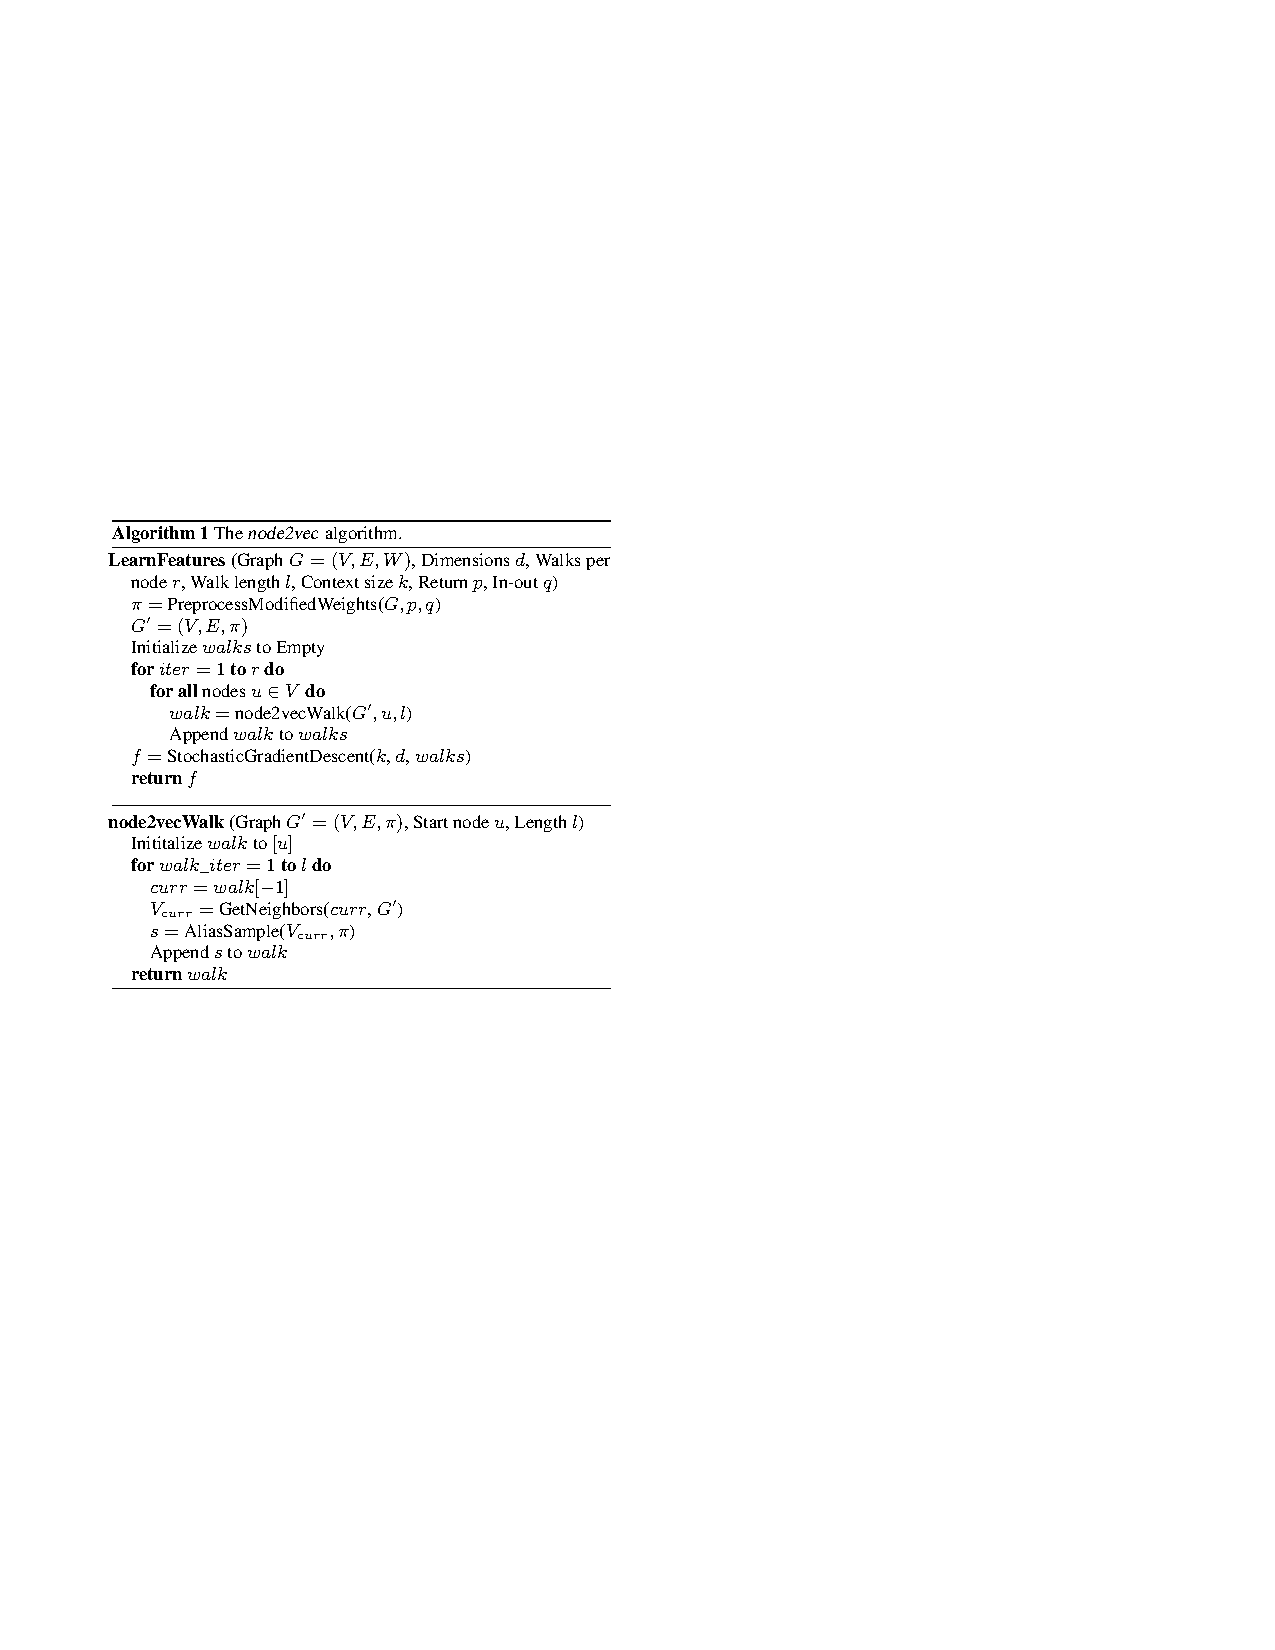
\includegraphics[height=5cm]{node2vec_3.pdf}
    \begin{corollary}
        $\max _{f} \sum_{u \in V}\left[\sum_{n_{i} \in N_{S}(u)} f\left(n_{i}\right) \cdot f(u)-\log Z_{u}\right]$
    \end{corollary}
\end{frame}
% 总结
\begin{frame}{Node2Vec}
    \framesubtitle{总结}
    \begin{columns}
        \begin{column}{0.5\textwidth}
            \centering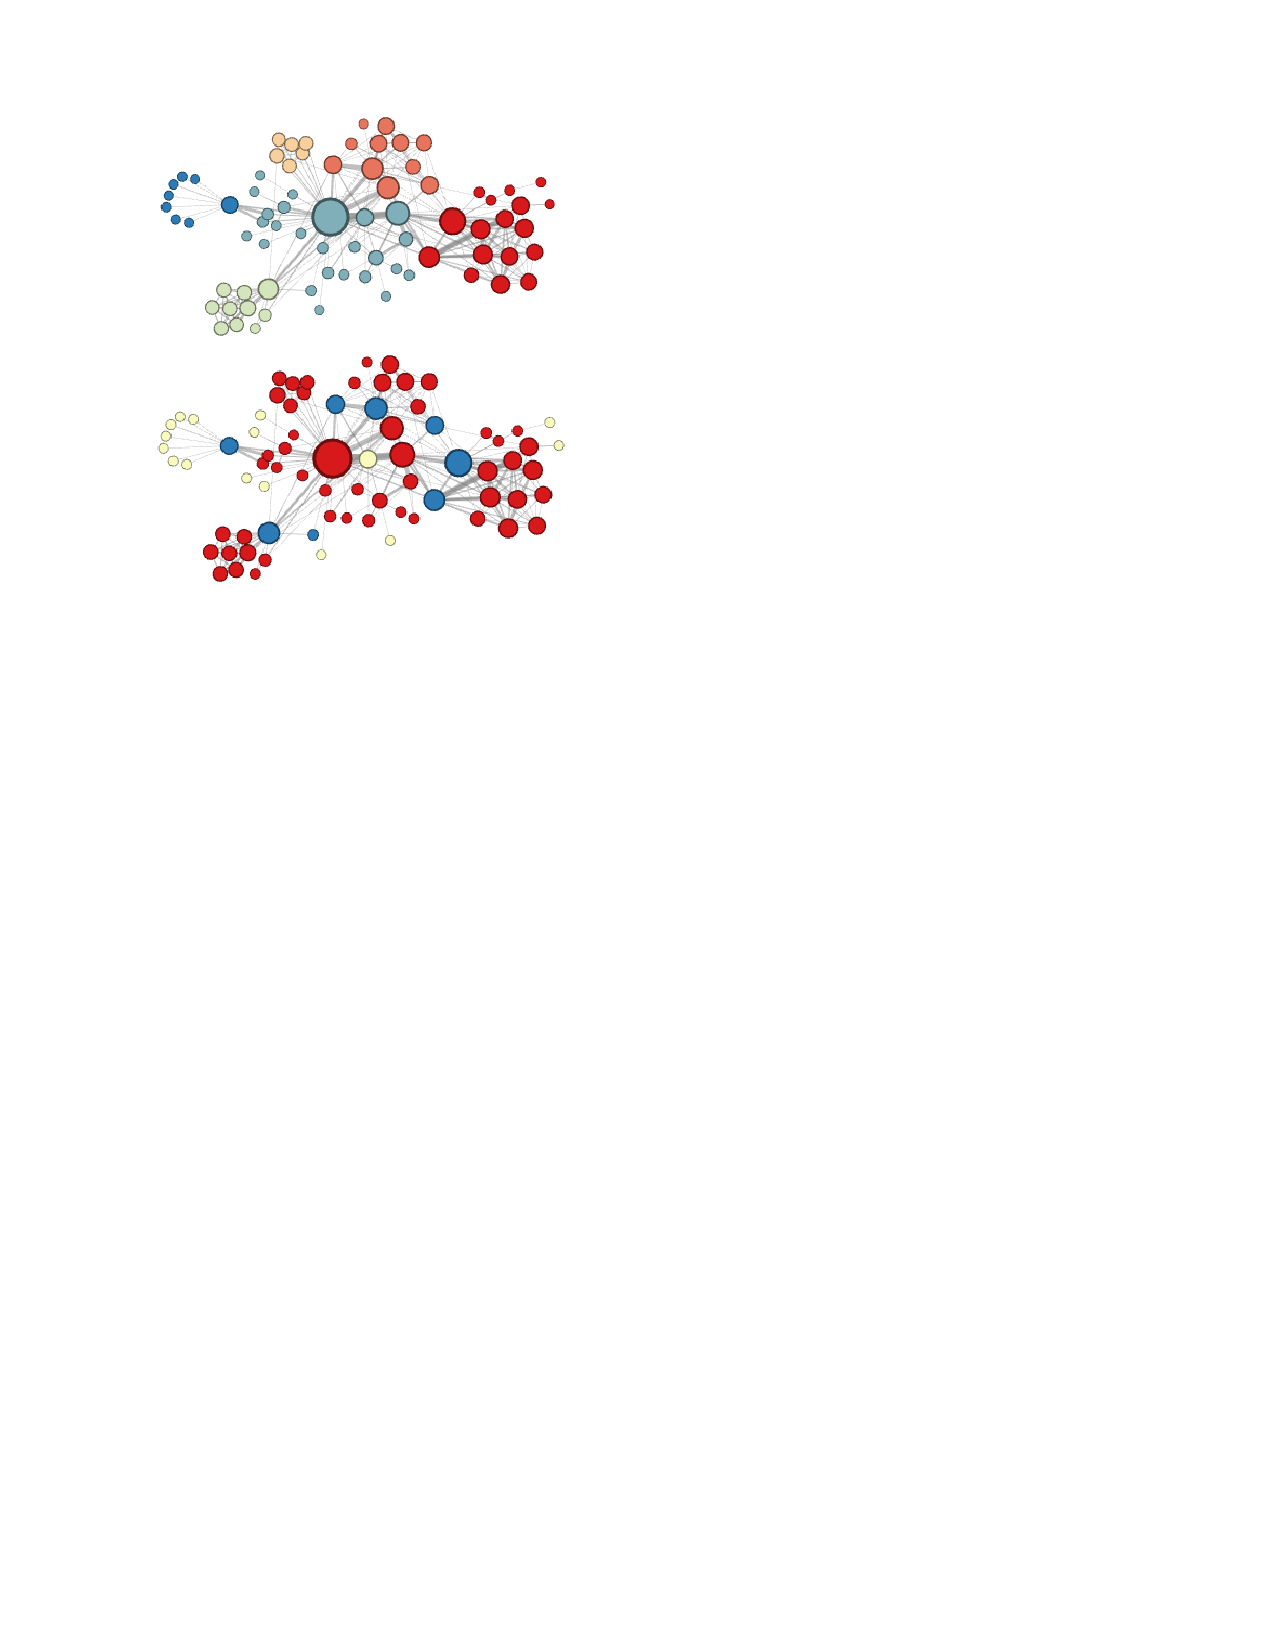
\includegraphics[width=\textwidth]{node2vec_4.pdf}
        \end{column}
        \begin{column}{0.5\textwidth}
            1.左图上半部分使用的参数$p > q$,相同社区的点都被划分成了相同的颜色,更多体现的是同质性;而下半部分则是$p < q$,更多的
            是结构相似的点被划分成了相同的颜色,更多体现的是结构相似性。\\
            2.Node2Vec本质就是通过BFS与DFS两种随机游走的策略来控制随机游走的方向以此来偏向捕获特定的相似性。
            3.Node2Vec也是有一些缺陷存在,例如如果两个点如果相距太远,很难通过游走策略来捕捉其结构相似性。
        \end{column}
    \end{columns}
\end{frame}
% ---------------------------------------Stuc2Vec---------------------------------------
\section{Struc2Vec}
% Overview
\begin{frame}{Struc2Vec}
    \centering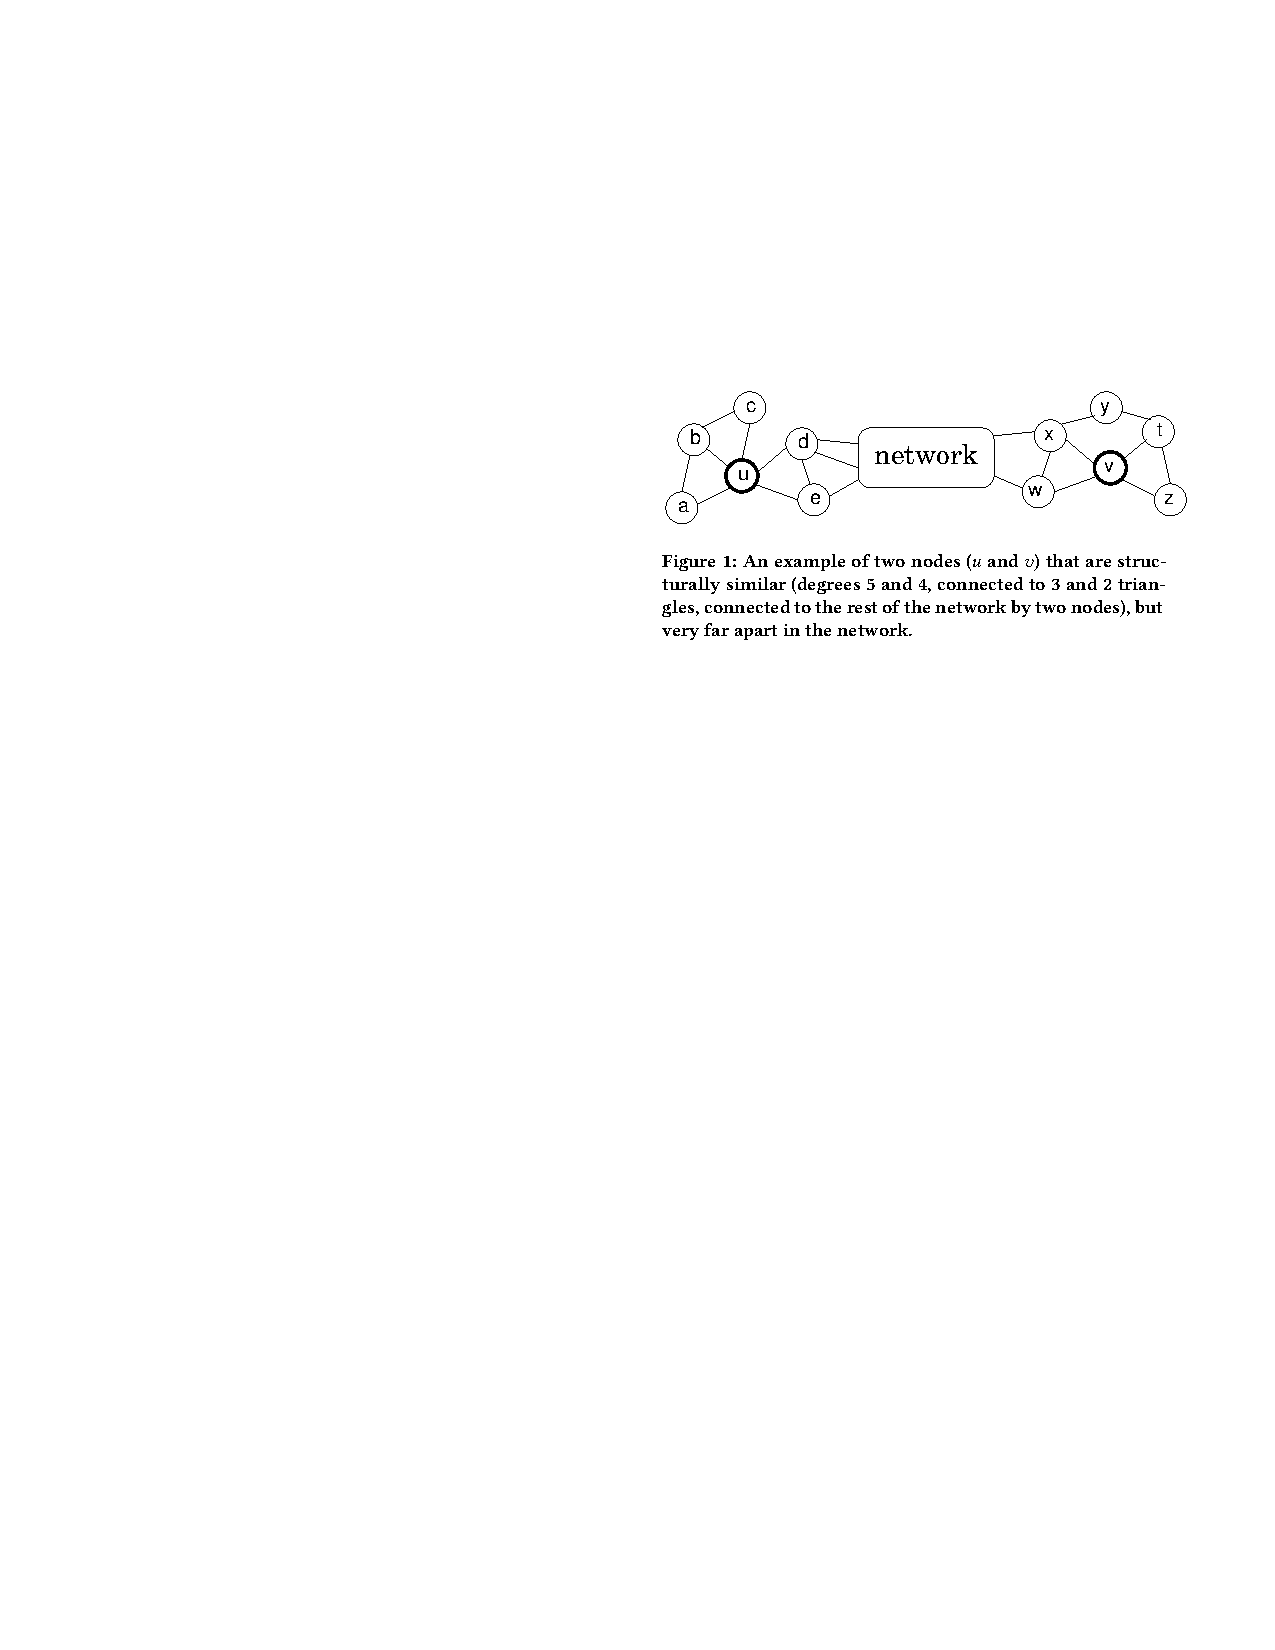
\includegraphics[height=5cm]{struc2vec.pdf}
    \begin{block}{Limitation}
        Structurally similar nodes will never share the same context if their distance (hop count) is larger than the Skip-Gram window.
    \end{block}
\end{frame}
% 符号解释
\begin{frame}{Struc2Vec}
    \framesubtitle{Structural Similarity}
    \begin{equation}
        \begin{gathered}
        f_{k}(u, v)=f_{k-1}(u, v)+g\left(s\left(R_{k}(u)\right), s\left(R_{k}(v)\right)\right) \\
        k \geq 0 \text { and }\left|R_{k}(u)\right|,\left|R_{k}(v)\right|>0
        \end{gathered}
    \end{equation}
    \begin{alertblock}{符号解释}
        \begin{description}
            \item [$f_k(u, v)$] structural distance when consider k-hop neighborhoods
            \item[$R_{k}(u)$] the ring of nodes at distance k
            \item[$s(S)$] the ordered degree sequence
            \item[$g(a, b)$] DTW Function  
        \end{description}
    \end{alertblock}
\end{frame}
% R, S
\begin{frame}{Struc2Vec}
    \framesubtitle{Example}
    \begin{columns}
        \begin{column}{0.5\textwidth}
            \centering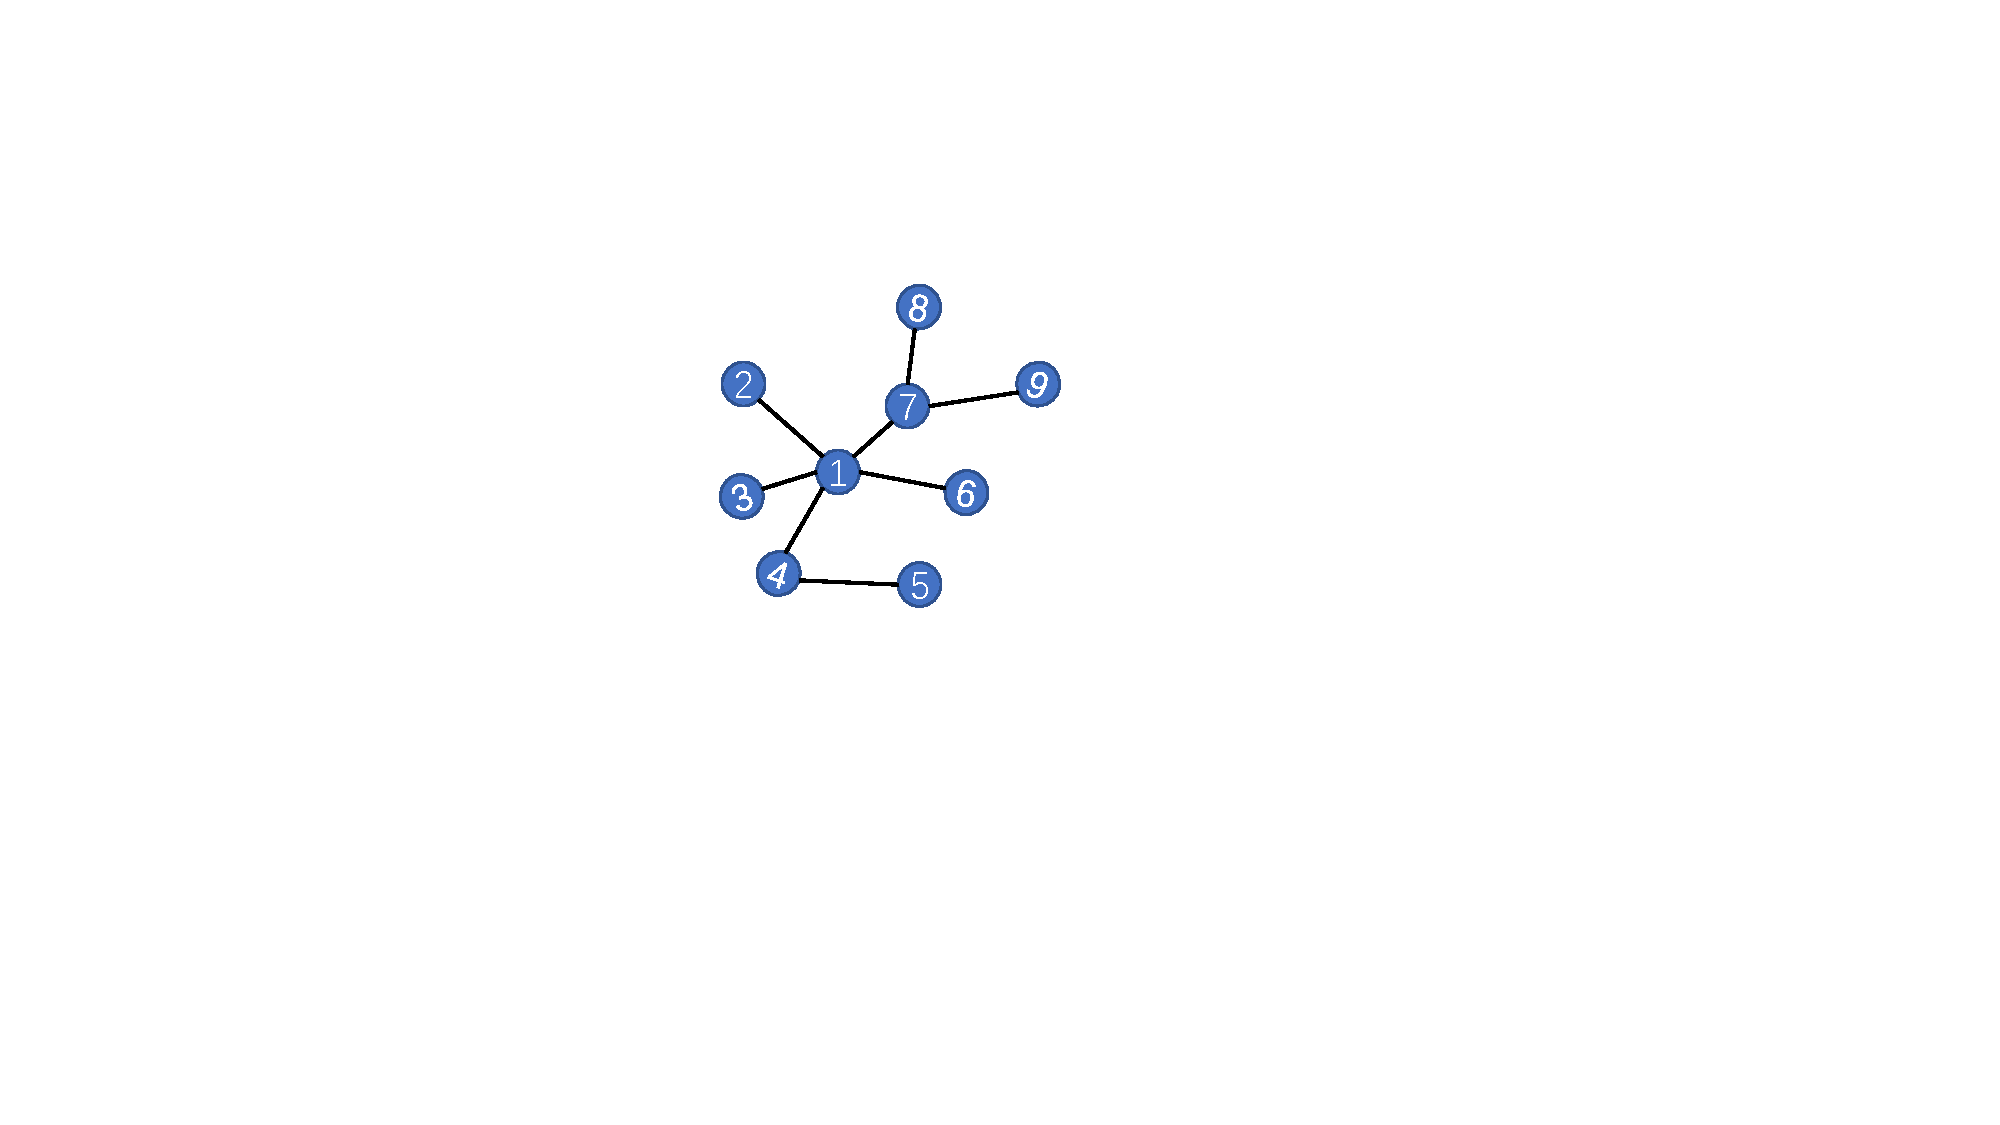
\includegraphics[height=4.6cm]{struc2vec_example.pdf}
        \end{column}
        \begin{column}{0.5\textwidth}
            \begin{example}
                \begin{align*}
                    & R_1(1)=\{2,3,4,6,7\} \\
                    & R_2(1)=\{5,8,9\}\\
                    & s(R_1(1))=\{1,1,1,2,3\}\\
                    & s(R_2(1))=\{1,1,1\} \\
                \end{align*}
            \end{example}
        \end{column}
    \end{columns}
\end{frame}
% DTW
\begin{frame}{Struc2Vec}
    \framesubtitle{DTW}
    \begin{block}{Dynamic Time Warping}
        利用动态规划的思想来计算两条不等长序列的相似度
    \end{block}
    动态转移方程如下:
    $$
    g(i, j) = min\{g(i-1, j),g(i, j-1),g(i-1, j-1)\} + d(i, j)
    $$
    $$d(a, b) = \frac{max(a, b)}{min(a, b)} - 1$$
\end{frame}
% 优化
\begin{frame}{Struc2Vec}
    \framesubtitle{Optimization}
    OPT1: 对于每一个节点的有序度序列,其空间复杂度为$O(n)$,为了减少花费,将其转化为(度数,出现次数)这样的形式,距离方程变成如下:
    $$
    \operatorname{dist}(a, b)=\left(\frac{\max \left(a_{0}, b_{0}\right)}{\min \left(a_{0}, b_{0}\right)}-1\right) \max \left(a_{1}, b_{1}\right)
    $$
    OPT2:两个度数相差很大的点没有必要计算他们的距离,使用双指针寻找与度相近的节点进行计算,将时间复杂度从$O(n^2)$降为$O(nlog(n))$\\
    OPT3:限制层次带权图层数
\end{frame}
%总结
\begin{frame}{Struc2Vec}
    \framesubtitle{总结}
    1. Struc2Vec基于节点之间的结构相似性来构建多层加权图,并在这张多层加权图上进行游走生成序列,使用Word2Vec的思想进行优化,
    不像Node2Vec受限于Window Size的限制导致无法捕捉距离很远的两个点之间的结构相似度\\
    2. 这篇文章的核心就是公式(4),通过计算两个节点之间的度序列的相似性来计算其结构相似性
\end{frame}
% ---------------------------------------LINE--------------------------------------------
\section{LINE}
% 一阶相似度与二阶相似度
\begin{frame}{LINE}
    \framesubtitle{Overview}
    \centering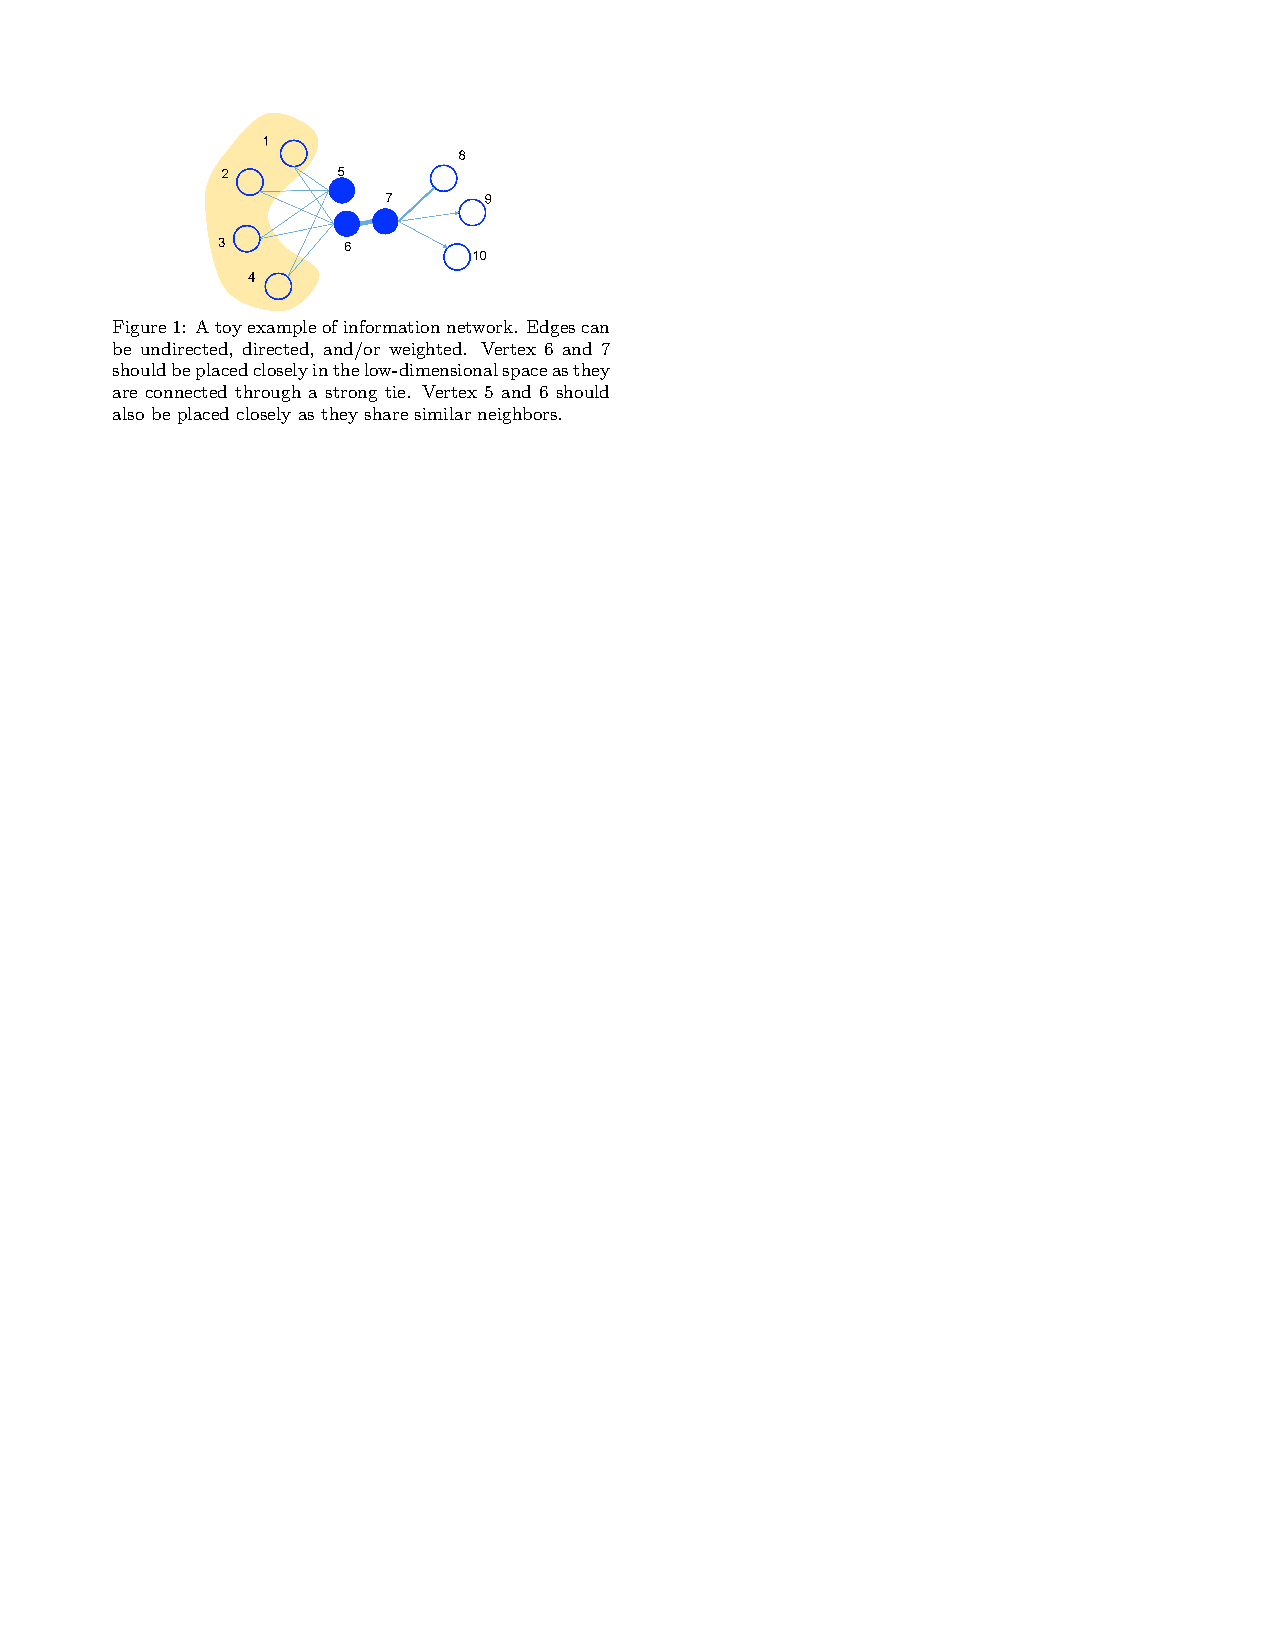
\includegraphics[height=6cm]{line.pdf}
\end{frame}
% 一阶
\begin{frame}{LINE}
    \framesubtitle{First-Order Proximity}
    The Joint Probability between $v_i$ and $v_j$:
    $$p_{1}\left(v_{i}, v_{j}\right)=\frac{1}{1+\exp \left(-\vec{u}_{i}^{T} \cdot \vec{u}_{j}\right)}$$ 
    Empirical Probability $\hat{p}_1(i, j)=\frac{w_{ij}}{W}$
    $$O_{1}=d\left(\hat{p}_{1}(\cdot, \cdot), p_{1}(\cdot, \cdot)\right)$$ 
    where $d(·, ·)$ is the distance between two distributions.
    \begin{block}{Objective Function}
        min $O_{1}=-\sum_{(i, j) \in E} w_{i j} \log p_{1}\left(v_{i}, v_{j}\right)$
    \end{block}
\end{frame}
% 二阶
\begin{frame}{LINE}
    \framesubtitle{Second-Order Proximity}
    The Probability of Context $v_j$ generated by vertex $v_i$ as:
    $$
    p_{2}\left(v_{j} \mid v_{i}\right)=\frac{\exp \left(\vec{u}_{j}^{T} \cdot \vec{u}_{i}\right)}{\sum_{k=1}^{|V|} \exp \left(\vec{u}_{k}^{\prime T} \cdot \vec{u}_{i}\right)}
    $$
    Empirical Probability $\hat{p}_1(v_j \mid v_i)=\frac{w_{ij}}{d_i}$
    \begin{block}{Objective Function}
        $O_{2}=-\sum_{(i, j) \in E} w_{i j} \log p_{2}\left(v_{j} \mid v_{i}\right)$
    \end{block}
\end{frame}
% 优化
\begin{frame}{LINE}
    \framesubtitle{Optimization}
    1. Negative Sample
    $$
    \log \sigma\left(\vec{u}_{j}^{\prime T} \cdot \vec{u}_{i}\right)+\sum_{i=1}^{K} E_{v_{n} \sim P_{n}(v)}\left[\log \sigma\left(-\vec{u}_{n}^{T} \cdot \vec{u}_{i}\right)\right]
    $$
    where $\sigma (x) = \frac{1}{1 + exp(−x)}$ is the sigmoid function.\\
    \hspace*{\fill}\\ 
    \hspace*{\fill}\\ 
    \hspace*{\fill}\\
    2. Edge Sample - Alias Sample
\end{frame}
% 总结
\begin{frame}{LINE}
    \framesubtitle{总结}
    1.LINE的核心思想是通过捕获图中的一阶相似度(两个点之间有连接)和二阶相似度(两个点有相同的邻居)\\
    2.使用KL散度来计算相似度,最小化条件概率与经验概率之间的差距\\
    3.对于一阶相似度,如果只计算两个向量的乘积会导致平凡解,因此也加入负采样的思想进行优化,这样就将一阶
    相似度与二阶相似度统一使用一个目标函数进行表示,唯一的差别就在于$u_j$,在优化一阶与二阶时对其使用不同
    的Embedding。
\end{frame}
% -----------------------------------------SDNE-----------------------------------------
\section{SDNE}
\begin{frame}{SDNE}
    \framesubtitle{Overview}
    \centering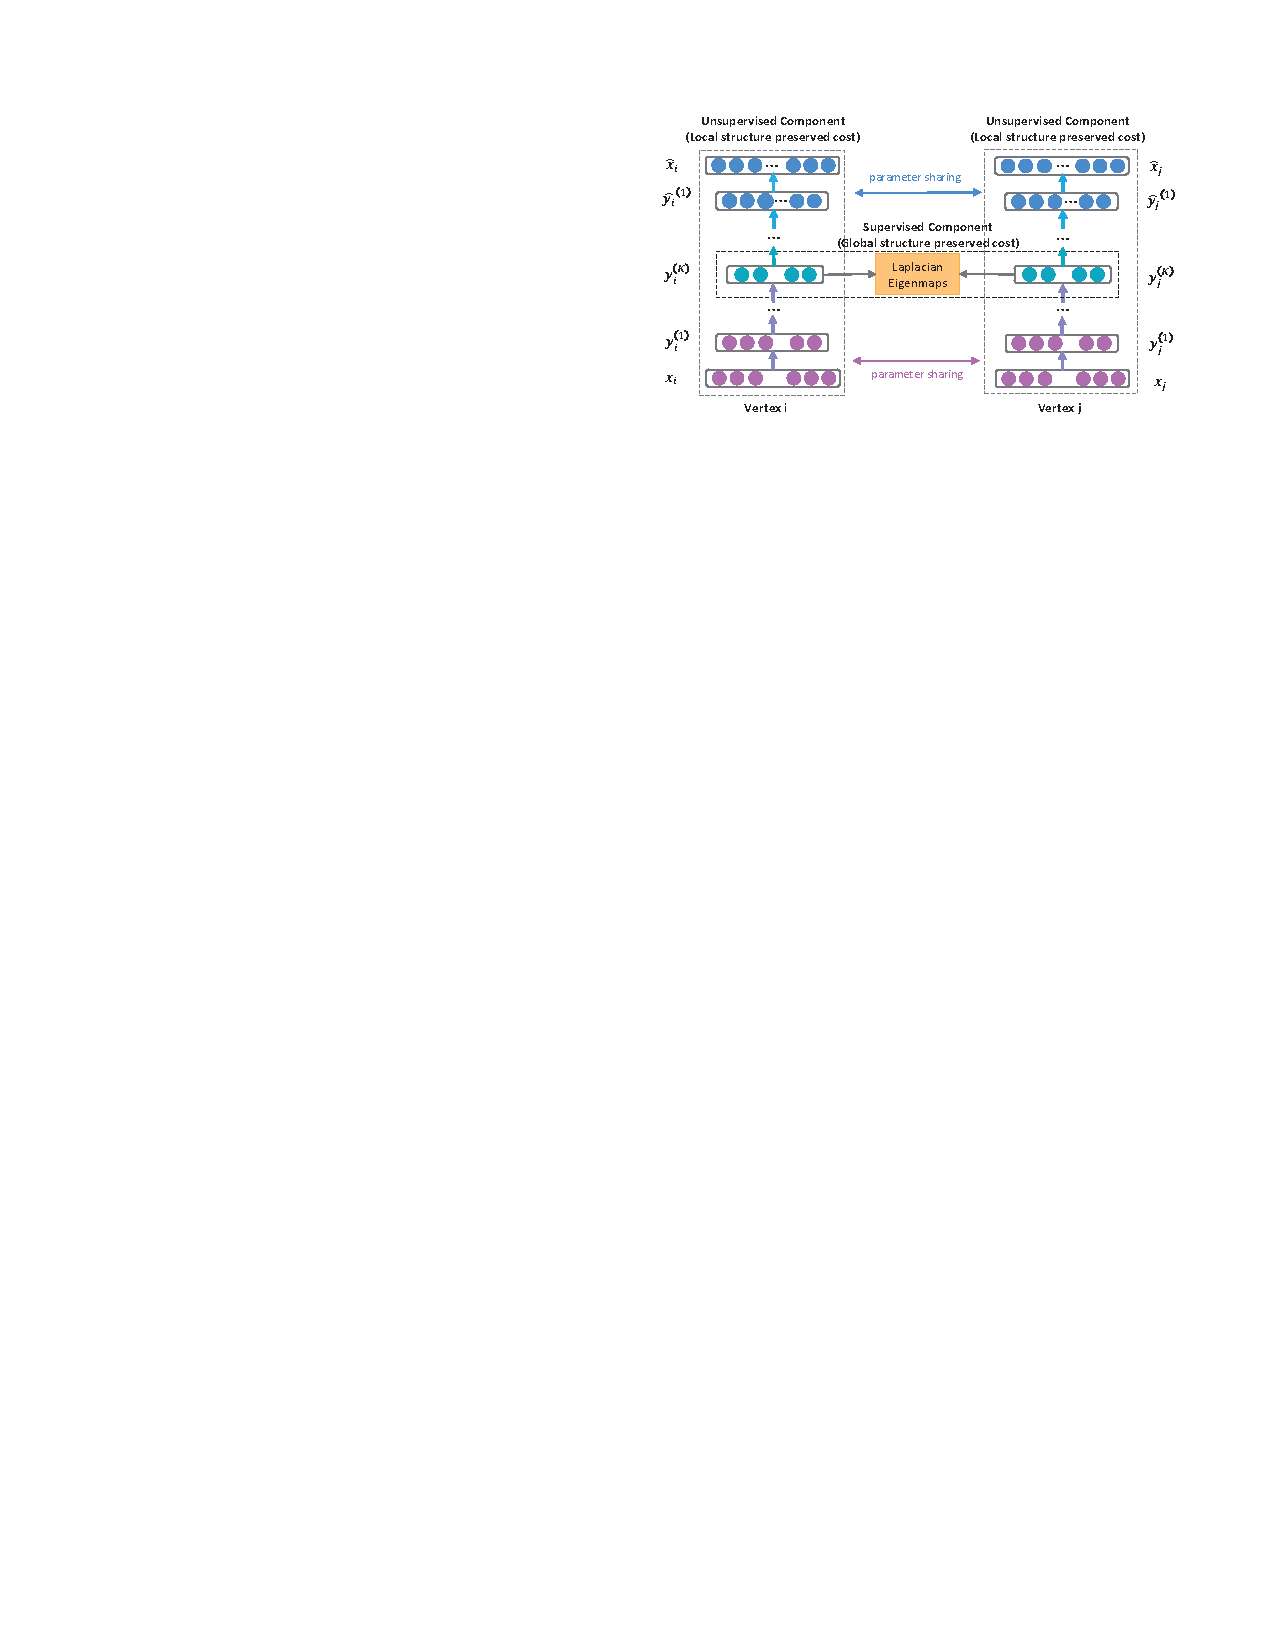
\includegraphics[height=6cm]{SDNE.pdf}
\end{frame}
% 一阶
\begin{frame}{SDNE}
    \framesubtitle{First-Order Proximity}
    Encoder and Decoder
    $$
    \begin{aligned}
    &\mathbf{y}_{i}^{(1)}=\sigma\left(W^{(1)} \mathbf{x}_{i}+\mathbf{b}^{(1)}\right) \\
    &\mathbf{y}_{i}^{(k)}=\sigma\left(W^{(k)} \mathbf{y}_{i}^{(k-1)}+\mathbf{b}^{(k)}\right), k=2, \ldots, K
    \end{aligned}
    $$
    First-Order Proximity Loss Function
    $$
    \begin{aligned}
    \mathcal{L}_{1 s t} &=\sum_{i, j=1}^{n} s_{i, j}\left\|\mathbf{y}_{i}^{(K)}-\mathbf{y}_{j}^{(K)}\right\|_{2}^{2} \\
    &=\sum_{i, j=1}^{n} s_{i, j}\left\|\mathbf{y}_{i}-\mathbf{y}_{j}\right\|_{2}^{2}
    \end{aligned}
    $$
\end{frame}
% 二阶
\begin{frame}{SDNE}
    \framesubtitle{Second-Order Proximity}
    The autoencoder goal is to minimize:
    $$
    \mathcal{L}=\sum_{i=1}^{n}\left\|\hat{\mathbf{x}}_{i}-\mathbf{x}_{i}\right\|_{2}^{2}
    $$
    {Structural Similarity $x_i=s_i$} 
    $$
    \begin{aligned}
    \mathcal{L}_{2 n d} &=\sum_{i=1}^{n}\left\|\left(\hat{\mathbf{x}}_{i}-\mathbf{x}_{i}\right) \odot \mathbf{b}_{\mathbf{i}}\right\|_{2}^{2} \\
    &=\|(\hat{X}-X) \odot B\|_{F}^{2}
    \end{aligned}
    $$
\end{frame}
% 损失函数
\begin{frame}{SDNE}
    \framesubtitle{Objective Function}
    正则化部分
    $$
    \mathcal{L}_{r e g}=\frac{1}{2} \sum_{k=1}^{K}\left(\left\|W^{(k)}\right\|_{F}^{2}+\left\|\hat{W}^{(k)}\right\|_{F}^{2}\right)
    $$
    损失函数
    $$
    \begin{aligned}
    \mathcal{L}_{m i x} &=\mathcal{L}_{2 n d}+\alpha \mathcal{L}_{1 s t}+\nu \mathcal{L}_{r e g} \\
    &=\|(\hat{X}-X) \odot B\|_{F}^{2}+\alpha \sum_{i, j=1}^{n} s_{i, j}\left\|\mathbf{y}_{i}-\mathbf{y}_{j}\right\|_{2}^{2}+\nu \mathcal{L}_{r e g}
    \end{aligned}
    $$
\end{frame}
% 总结
\begin{frame}{SDNE}
    \framesubtitle{总结}
    1.DeepWalk使用随机游走与Skip-Gram来学习节点表示,但是缺少一个明确的优化函数来学习图结构特征,LINE只是结合了
    一阶相似度与二阶相似度,其节点表示受限于它是一个浅层模型效果不够好。\\
    2.SDNE的构建思路围绕三点:模型的高度非线性来更好的学习节点的深层次表示;能够很好的保留结构特性;如何处理稀疏性问题。\\
    3.SDNE使用自编码器来优化二阶相似度(其中输入$x$是度序列,跟Struc2Vec一样都是通过度序列来计算结构上的相似度),
    使得结构相似的顶点具有相似的Embedding,而对于一阶相似度则是使得相邻两个顶点对应的Embedding接近。
\end{frame}
% 复现结果
\section{Experiment}
\begin{frame}{复现结果}
    \begin{table}[]
        \begin{tabular}{|l|l|l|l|l|}
        \hline
        Dataset       & Method    & LabelNode & macro-F1 & 参考值 \\ \hline
        Wiki          & Node2Vec  & 50\%      & 51.10    & 50.52  \\ \hline
                      & SDNE      & 50\%      & 49.70    & 49.80  \\ \hline
        BlogCatalog   & DeepWalk  & 50\%      & 21.80    & 21.10  \\ \hline
                      & Node2Vec  & 50\%      & 23.50    & 23.00  \\ \hline
        Wikipedia     & LINE      & 50\%      & 11.40    & 11.64  \\ \hline
        Brazil-Flight & Struc2Vec & 50\%      & 67.94    & 68.30  \\ \hline
        \end{tabular}
    \end{table}
\end{frame}
% -----------------------------------------END------------------------------------------
\end{document}